
\documentclass[runningheads]{llncs}
\usepackage[T1]{fontenc}
\usepackage[utf8]{inputenc}
\usepackage{graphicx}
\usepackage{amsmath,amssymb}
\usepackage{booktabs,longtable,array,calc}
\usepackage{hyperref}
\usepackage{microtype}
\usepackage{tabularx}
\usepackage{booktabs}
\usepackage{float}
\usepackage{caption}
\usepackage{caption}
\captionsetup{
    font=small
}
\usepackage[
    font=footnotesize,
    labelfont=bf
]{caption}

\usepackage{titlesec}

\titlespacing*{\section}
{0pt}{2.0ex plus 0.8ex minus 0.3ex}{1.2ex}

\titlespacing*{\subsection}
{0pt}{1.5ex plus 0.5ex minus 0.2ex}{0.8ex}

\renewcommand{\figurename}{Figure}

\captionsetup[figure]{skip=2pt}
\captionsetup[table]{skip=2pt}
\setlength{\textfloatsep}{4pt}
\setlength{\floatsep}{2pt}
\setlength{\intextsep}{2pt}
\setlength{\abovedisplayskip}{1pt}
\setlength{\belowdisplayskip}{1pt}

\usepackage{bm}

\providecommand{\tightlist}{\setlength{\itemsep}{0pt}\setlength{\parskip}{0pt}}
\newcommand{\real}[1]{#1}

\begin{document}
\title{Physics-Informed Closure Learning for Reduced Radiotherapy Tumor Dynamics}
\titlerunning{Physics-Inspired Closure Learning}
\author{Paweł Jarosz\and Igor Zakrocki\and Witold Dzwinel}
\authorrunning{P. Jarosz et al.}
\institute{AGH University of Krakow, WI Department of Computer Science\\
\email{\{zakrocki@student.agh.edu.pl, pawjarosz@student.agh.edu.pl, dzwinel@agh.edu.pl\}}}
\maketitle
\begin{abstract}
High-fidelity radiotherapy models based on spatio-temporal partial
differential equations are computationally too expensive for interactive
therapy-planning systems and emerging Language--Driven Therapy Design
frameworks based on LLMs and RAG architectures. In this work, we
investigate whether physics-informed machine learning methods can
compensate for information loss introduced during aggressive reduction
of spatial tumor models to low-dimensional ordinary differential
equation (ODE) surrogates.
We compare classical ODE surrogates, purely data-driven Neural ODEs
(NODEs), and physics-informed residual neural models (PI-NODEs) in
radiotherapy scenarios involving incomplete overlap between tumor and
irradiation regions. The proposed PI-NODE combines a mechanistic
radiotherapy model with a learnable residual closure term.
The results demonstrate that reduced ODE surrogates absorb unresolved
spatial effects into distorted effective parameters, while purely
data-driven NODEs exhibit limited extrapolation stability. In contrast,
the proposed PI-NODE formulation preserves physically interpretable
parameters while partially reconstructing unresolved spatial dynamics
eliminated during PDE-to-ODE reduction.

Beyond the controlled phantom, we evaluate the same formulations on
117 real glioma patients, using each patient's own anatomy, tumor
segmentation and imaging-derived invasiveness to drive a three-dimensional
reaction--diffusion reference with a grafted radiotherapy field. The central
claim is confirmed and strengthened: where the irradiation field is under-sized
or displaced, a learned closure forecasts recurrence two to three times more
accurately than any purely mechanistic surrogate. Three further findings concern
the weights themselves. First, $\omega$ and $s_{r}$ are exact gauge freedoms
rather than mixing coefficients --- which is why they cannot be normalized to
sum to one --- and a sweep confirms it operationally: varying $s_{r}$ tenfold
leaves the realized physics/machine-learning balance unchanged while changing
accuracy substantially. Second, the published weights are not the best cell of
their own grid, and the setting that wins realizes $90\,\%$ machine learning,
so the formulation performs best as a lightly-anchored neural ODE rather than as
a balanced hybrid. Third, we give a convex, bounded and anchored replacement
whose single coefficient is calibrated to the realized balance and spans the
full range, and we quantify what that identifiability costs in accuracy.

\keywords{Physics-informed machine learning \and Neural ODE \and Surrogate modeling \and Radiotherapy \and Data assimilation \and Identifiability}
\end{abstract}

% ==========================================================================
% Body. Each file is one top-level section; edit them directly.
% ==========================================================================
% ==========================================================================
% Introduction
% ==========================================================================

\section{Introduction}

Modern oncology increasingly relies on computational models for
predicting tumor evolution and optimizing anticancer therapies. In
particular, recent advances in Large Language Models (LLMs) and
Retrieval-Augmented Generation (RAG) systems have opened the possibility
of developing interactive frameworks for Language--Driven Therapy Design
(LDTD), where clinicians can explore treatment scenarios and control
predictive simulations through natural language \cite{reka2026conversational}. However, practical
implementation of such systems requires simulation engines operating in
near real-time, which remains infeasible for complex mechanistic tumor
models involving high-dimensional spatial dynamics and computationally
expensive partial differential equations.

A natural solution is the use of surrogate models that approximate the
behavior of detailed mechanistic simulations at a much lower
computational cost. Nevertheless, aggressive model reduction -
especially the elimination of spatial information - introduces
substantial challenges. Reduced ordinary differential equation (ODE)
models frequently fail to capture important effects arising from tumor
geometry, spatial heterogeneity, and mismatches between tumor and
treatment-field geometry. As a consequence, unresolved spatial dynamics
are often absorbed into distorted effective model parameters, leading to
biased predictions and reduced interpretability.

In this work, we investigate whether simple physics-informed surrogate
models are capable of partially reconstructing the effects of neglected
spatial dynamics despite operating in a drastically simplified
non-spatial representation. We focus on radiotherapy-driven tumor
dynamics (e.g. \cite{Balcerak2025GliODIL}, \cite{sun2025physicsinformed}, \cite{Sujitha2023RadiotherapyBrainTumor}) in scenarios where the irradiation field only partially
overlaps with the tumor volume or becomes spatially shifted with respect
to the evolving tumor geometry during repeated treatment fractions. Such
situations naturally generate unresolved effects including asymmetric
survival regions, delayed recolonization of irradiated areas, outward
invasive expansion, and spatially heterogeneous regrowth dynamics.
The presented framework is intended as a controlled computational
testbed for investigating whether physics-informed surrogate models can
reconstruct unresolved spatial effects eliminated during PDE-to-ODE
reduction. From the Scientific Machine Learning perspective, the
PI-NODE architecture may also be interpreted as a reduced-order
UDE-based \cite{rackauckas2019diffeqflux} closure model designed to compensate for unresolved spatial
dynamics introduced by aggressive PDE-to-ODE reduction including spatially heterogeneous radiation damage accumulation,
asymmetric post-treatment survival patterns, and delayed
recolonization fronts.

The experiments presented should therefore be interpreted primarily as a
methodological investigation of closure-aware surrogate modeling for
future interactive therapy-planning systems and Language–Driven Therapy
Design frameworks requiring computationally efficient predictive models.

% ==========================================================================
% Models of cancer dynamics under therapy
% ==========================================================================

\section{Models of Cancer Dynamics Under Therapy}
\label{sec:models}
\subsection{Spatial Model}
There is a plethora of cancer models based on various modeling paradigms
(see e.g., \cite{cristini2010multiscale}, \cite{Sekyere2025VascularTumor}, \cite{wcislo20093}). Most of them concern only the
phase of tumor growth. Much less consider various anti-cancer therapies
(see e.g. \cite{Sujitha2023RadiotherapyBrainTumor}, \cite{dzwinel2021supermodeling}). Let us assume that we have an array of such
models ordered in decreasing complexity starting from the reality R: R
\(\rightarrow\)$M_{\infty} \to \ldots \to M_i \to M_{i-1} \to \ldots \to M_1 \to M_0$.
We assume that the number of parameters will decrease from the most
complicated to the simplest model. Let us assume that $M_{\infty}$
is the most faithful metaphor of reality R, while possible differences
come from various sources of uncertainty. In general, even in reality,
assuming the same two initial setups, one can obtain (after some time)
different outcomes resulting from the nonlinear amplification of small
variations in the systems (chaotic behavior). Due to the measurement,
numerical, and round-off errors the same situation may happen for
computer simulations. So, here, before introducing the reduced formulation, we consider a more
general radiotherapy-driven reaction-diffusion model $M_{2}$ in which tumor
evolution is coupled with treatment response, oxygen-dependent
radiosensitivity, and unresolved microenvironmental effects. In its
compact form, such a model may be written as \cite{Sujitha2023RadiotherapyBrainTumor}:
\begin{equation}
\label{eq:pde_general}
\begin{split}
    \frac{\partial u(x,t)}{\partial t}
&=
\nabla \cdot \left( D(x)\nabla u \right)
+
F_{b}(u,x,t;\theta_{b})
-
U(t)\,G_{R}(u,R(x,t),h(x,t);\theta_{R}) \\
&+
\mathcal{M}(u,x,t).
\end{split}
\end{equation}
where \(u(x,t)\) denotes the local tumor cell density, \(D(x)\) is a
possibly heterogeneous diffusion coefficient, \(F\) represents intrinsic
tumor growth and tissue-limited proliferation, \(G_{R}\) describes
radiotherapy-induced cell killing modulated by the delivered dose
\(R(x,t)\)and local radiosensitivity factors \(h(x,t)\), while
\(\mathcal{M}\) collects additional microenvironmental mechanisms such as
hypoxia, vascular remodeling, delayed cell death, repair processes, and
repopulation between treatment fractions. Additionally, \(U(t)\) defines
the radiotherapy fractionation schedule, i.e. the sequence of
irradiation events. A convenient representation is
\begin{equation}
\label{eq:therapy_schedule}
U(t)
=
\sum_{k=1}^{N_f}
\delta_{\tau}(t-t_k).
\end{equation}
where \(N_{f}\) is the total number of fractions, \(t_{k}\) denotes the
time of the \(k\)-th irradiation, and \(\delta_{\tau}(t - t_{k})\) is a
narrow temporal pulse representing dose delivery over a short time
interval. A simplified instance of this general formulation is then obtained by
assuming logistic tumor growth, constant diffusion, multiplicative
radiotherapy-induced killing, and representing all unresolved effects by
a residual term \cite{Sujitha2024ChemoRadiotherapy}:
\begin{equation}
\label{eq:pde_simplified}
\frac{\partial u(x,t)}{\partial t}
=
D\nabla^{2}u
+
\rho u\left(1-\frac{u}{K}\right)
-
\beta U(t)R(x)H(x)u
+
\xi(u,x,t).
\end{equation}
where: \(\rho\) denotes the intrinsic tumor proliferation rate,
\(K\) is the effective carrying capacity,
\(\beta\) Radiosensitivity coefficient, the residual term \(\xi(u,x,t)\) represents unresolved biological
mechanisms and modeling uncertainties.

\subsection{ODE Model}

In practice, 3D tumor structure can be observed using imaging techniques
such as CT or MRI; however, these observations are limited to discrete
snapshots separated by relatively large time intervals. Consequently,
the full spatio-temporal field \(u(x,t)\) is not directly observable.
Moreover, clinical measurements typically capture only the visible tumor
volume, which may underestimate the true tumor burden due to limited
resolution and the presence of diffuse or microscopic disease. In
reduced models, this discrepancy can be partially compensated by
introducing an effective tumor mass, for example by incorporating safety
margins or scaling factors. So, instead, measurements typically
correspond to macroscopic quantities. Therefore, we introduce an
observable such as tumor mass as:
\begin{equation}
\label{eq:mass}
y(t)
=
\int_{\Omega} u(x,t)\,dx
\qquad \text{and} \qquad
\int_{\Omega} \nabla^{2}u\,dx = 0
\end{equation}
assuming zero-flux BC. Combining Equation (\ref{eq:pde_simplified}) and  Equation (\ref{eq:mass}):
\begin{equation}
\dot y=
\rho y
-\frac{\rho}{K}\int_\Omega u^2dx
-\beta\int_\Omega URHu\,dx
+\int_\Omega \xi\,dx .
\end{equation}
If we now wish to approximate it using a logistic ODE:
\(ay - by^{2} = ay(1 - \frac{b}{a}y)\) in combination with radiotherapy,
e.g.
\begin{equation}
\small
\begin{aligned}
\dot y
&=
\dot y = ay - by^2 - cU(t)\bar R_{\mathrm{eff}}(t)y
\\
\delta(t)
&=
-\frac{\rho}{K}
\Bigl(\int_\Omega u^2dx-\alpha y^2\Bigr)
-\beta
\Bigl(
\int_\Omega U(t)RHu\,dx
-\bar R_{\mathrm{eff}}(t)y
\Bigr)
+\int_\Omega \xi(u,x,t)\,dx .
\end{aligned}
\end{equation}
where:
\begin{itemize}
    \item $R(x,t)$ local radiotherapy at PDE.

    \item $\bar R_{\mathrm{eff}}(t) = \frac{\int_{\Omega}^{}{R(x,t)H(x)u(x,t)\text{\,}dx}}{\int_{\Omega}^{}{u(x,t)\text{\,}dx}}$ - state-dependent exact effective mean

    \item the available macroscopic input used in ODE/NODE.
    
\end{itemize}

This is a very powerful example, as it highlights three sources of
error:
\begin{enumerate}
\item \emph{Spatial non-linearity}
\begin{equation}
\int_{\Omega} u^{2}\,dx
\neq
\alpha y^{2}
\end{equation}
\item \emph{Inconsistent response to radiotherapy}
\begin{equation}
\int_{\Omega} R(x,t)H(x)u\,dx
\neq
\bar{R}_{\mathrm{eff}}(t)\,y
\end{equation}
\item \emph{Missing physics / biology}
\begin{equation}
\int_{\Omega} \xi(u,x,t)\,dx
\neq 0
\end{equation}
\end{enumerate}
Let the ODE surrogate therefore take the ODE system form:

\begin{equation}
\label{eq:pinode_residual}
\frac{dy}{dt}
=
f_{RT}\!\left(y,U(t);\theta\right)
+
g_{\phi}\!\left(y,t,U(t)\right)
\end{equation}
\(y(t)\) - the system state (e.g., tumor mass, or an extended
state in NODE),
\(f_{RT}\) - the known mechanistic core (radiotherapy-driven dynamics),
\(g_{\phi}\) - a learned correction term accounting for unresolved
effects,
\(U(t)\) - the control/input function, describing the applied therapy
over time.

In our case:
\begin{equation}
\label{eq:frt}
f_{RT}(y,U(t);\theta)
=
\rho\,y(1-y)
-
\beta\,\overline{R}_{\mathrm{eff}}(t)\,U(t)\,y
\end{equation}
The $g_{\phi}$ -- learned correction, which depends on: the
complete cell distribution, the complete dose distribution, the
microenvironment, treatment history. Therefore, it compensates for:
(a) spatial heterogeneity of the dose,
(b) hypoxia,
(c) delayed cell death,
(d) repopulation between fractions,
and (e) other unmodelled processes.
Thus, \(g_{\phi}\) accounts for unresolved effects, while the treatment
itself is represented explicitly by the control function \(U(t)\).

% ==========================================================================
% Surrogate models
% ==========================================================================

\section{Surrogate Models}
\label{sec:surrogates}

The objective of this section is to investigate whether low-dimensional
surrogate models can reproduce selected effects of complex spatial
radiotherapy dynamics after PDE-to-ODE reduction and loss of spatial
information.
We compare three surrogate formulations of increasing complexity:
(i) a mechanistic two-state ODE calibrated through data assimilation,
(ii) a purely data-driven Neural ODE (NODE), and
(iii) a physics-informed residual PI-NODE combining mechanistic
radiotherapy dynamics with a learnable neural closure term.
The comparison focuses on how these approaches capture unresolved
effects associated with tumor--beam mismatch, incomplete irradiation
overlap, and delayed post-treatment dynamics.

To investigate robustness under observational uncertainty, additional
training ensembles were generated by perturbing the sparse observations
with Gaussian noise. Independent surrogate realizations were then
trained for each noisy observation set, producing probabilistic bundles
of trajectories and uncertainty bands for ODE, NODE, and PI-NODE models.

\subsection{Data Assimilation to a Reduced Two-State ODE Model}

As the first surrogate modeling strategy, we consider a reduced-order
two-state ordinary differential equation (ODE) system describing the
evolution of the normalized tumor mass together with an auxiliary latent
radiation-damage variable. The purpose of this model is to provide a
minimal mechanistic approximation of the spatial radiotherapy dynamics
generated by the reference PDE system while preserving delayed treatment
effects and multi-fraction memory.

The reduced surrogate is formulated as:
\begin{equation}
\label{eq:ode_rt_2state}
\dot y=\rho y(1-y/K_{\mathrm{eff}})-\gamma zy-\mu y,
\quad
\dot z=-z/\tau+U(t).
\end{equation}
where: \(z(t)\) is a latent accumulated radiation-damage variable, $\gamma$ is radiation-induced decay coefficient
\(\mu\) represents background decay,
and \(\tau\) is the characteristic damage relaxation time.

Unlike the earlier single-state formulation, the introduction of the
latent variable \(z(t)\) enables the surrogate to reproduce delayed
responses and cumulative effects associated with repeated irradiation
fractions. In particular, the second equation acts as a low-dimensional
memory mechanism integrating previous dose delivery.
The surrogate parameters
$\theta =
(\rho,\gamma,K,\mu,\tau)$
are estimated through data assimilation \cite{heaney2024dataassimilation} using synthetic observations
generated by the spatial PDE reference model. However, the reduced surrogate parameters should not be interpreted as physically identifiable quantities, but rather as effective closure-compensating coefficients. This affects all surrogates described in this paper. The assimilation objective is formulated as a nonlinear least-squares
optimization problem:
\begin{equation}
\label{eq:ode_training}
\theta^{*}
=
\arg\min_{\theta}
\mathcal{L}_{ODE}(\theta),
\qquad
\mathcal{L}_{ODE}(\theta)
=
\sum_{i=1}^{N_t}
\left(
y_{ODE}(t_i;\theta)
-
y_{PDE}(t_i)
\right)^2.
\end{equation}
Here, \(y_{PDE}(t_i)\) denotes the tumor mass extracted from the spatial
PDE reference simulation, whereas
\(y_{ODE}(t_i;\theta)\) is the corresponding reduced-order surrogate
prediction.
The optimization was performed using a hybrid strategy combining global
differential-evolution initialization followed by bounded local
gradient-based refinement. Assimilation was carried out only on sparse
synthetic observations sampled within a restricted temporal observation
window, while the remaining time interval was used for forecasting and
generalization assessment.

Due to the low dimensionality of the mechanistic surrogate, standard
nonlinear least-squares assimilation was sufficient in the present
study. For larger mechanistic systems with higher-dimensional parameter
spaces, more advanced assimilation approaches such as adjoint-based,
Bayesian, or ensemble methods may become necessary
\cite{heaney2024dataassimilation}.
\subsection{Classical Neural ODE (NODE) Surrogate}

While reduced mechanistic ODE surrogates provide an interpretable
approximation of the spatial tumor dynamics, their predictive capability
remains limited by the loss of spatial information during PDE-to-ODE
reduction. In particular, unresolved effects associated with
tumor--beam geometry mismatch, asymmetric irradiation, delayed treatment
response, and nonlocal spatial interactions cannot be represented
explicitly within fixed low-dimensional mechanistic models.

In the present work, the NODE surrogate \cite{chen2018neural}, \cite{rackauckas2020ude}, \cite{rubanova2019latent} is formulated as a two-state
continuous-time dynamical system:
\begin{equation}
\label{eq:node}
\dot y=f_{\psi}^{(y)}(y,z,t,U),
\qquad
\dot z=f_{\psi}^{(z)}(y,z,t,U).
\end{equation}
where:
\(f_{\psi}=(f_{\psi}^{(y)},f_{\psi}^{(z)})\) denotes a neural network
parameterized by trainable weights \(\psi\). The second latent state represents unresolved treatment-induced damage dynamics.
The latent state $z(t)$ provides low-dimensional treatment memory and delayed-response dynamics.

The neural network acts as a continuous-time nonlinear dynamical
operator approximating the temporal evolution of the reduced latent
state. In the present study, a fully connected feed-forward
architecture was employed consisting of:
\begin{itemize}
\item
an input layer containing $(y,z,t,U(t))$,
\item
two hidden layers with ReLU activation functions,
\item
a two-dimensional output representing the time derivatives $(dy/dt,dz/dt)$.
\end{itemize}
The final network layer was initialized close to zero in order to
stabilize early-stage trajectory integration and avoid unrealistically
large initial vector fields. Trajectory prediction was obtained through explicit time integration of
the learned neural dynamical system using a fourth-order Runge--Kutta
scheme. The NODE parameters were estimated by minimizing the trajectory mismatch
with respect to the PDE-generated observations:
\begin{equation}
\label{eq:node_training}
\psi^{*}
=
\arg\min_{\psi}
\mathcal{L}_{NODE}(\psi),
\qquad
\mathcal{L}_{NODE}
=
\sum_{i=1}^{N_t}
\left(
y_{NODE}(t_i)
-
y_{PDE}(t_i)
\right)^2.
\end{equation}
Only sparse observations from a restricted temporal assimilation window
were used during training, whereas the remaining time interval served as
an out-of-sample forecasting region for evaluating extrapolation
capability.
Although NODE surrogates offer substantially higher flexibility than
fixed mechanistic reduced-order models, they do not explicitly preserve
physical interpretability and may exhibit unstable extrapolation
behavior outside the assimilation interval, particularly under sparse
training conditions.

\subsection{Physics-Informed Neural ODE (PI-NODE) Surrogate}

To combine mechanistic interpretability with the flexibility of neural
correction terms, we introduce a physics-informed residual Neural ODE
(PI-NODE) surrogate. The proposed formulation augments the reduced
two-state mechanistic radiotherapy model with a learnable neural
closure term accounting for unresolved effects eliminated during the
PDE-to-ODE reduction process.

The PI-NODE surrogate augments the mechanistic reduced radiotherapy
model with a learnable neural residual closure term:
\begin{equation}
\label{eq:pinode_weighted}
\dot y
=
\omega f^{(y)}_{\mathrm{RT}}(y,z,U;\theta)
+
s_r g_{\psi}(y,z,t,U),
\qquad
\dot z
=
f^{(z)}_{\mathrm{RT}}(z,U;\theta),
\end{equation}
where
\(f^{(y)}_{\mathrm{RT}}\)
and
\(f^{(z)}_{\mathrm{RT}}\)
denote the mechanistic tumor-growth and latent damage dynamics defined
by Eq.~\eqref{eq:ode_rt_2state}.
Here:
\(\theta=(\rho,\gamma,K,\mu,\tau)\)
contains the mechanistic model parameters,
\(g_{\psi}\) denotes the neural residual closure term with trainable
parameters \(\psi\),
\(\omega\) controls the contribution of the mechanistic tumor dynamics,
and \(s_r\) scales the neural residual correction.

The residual neural component can be interpreted as a learned
reduced-order UDE closure model compensating for unresolved spatial
dynamics eliminated during PDE-to-ODE reduction, including:
incomplete overlap between tumor and irradiation regions,
delayed recolonization of irradiated areas,
outward expansion of untreated tumor regions,
nonlocal spatial effects,
and unresolved geometric heterogeneity.

In the present implementation, the neural residual correction is applied
only to the tumor evolution equation, whereas the latent damage
dynamics remain fully mechanistic.
Unlike the pure NODE formulation, the PI-NODE framework preserves
physically interpretable mechanistic parameters while allowing
unresolved dynamics to be reconstructed through residual learning.

The residual network employs the same feed-forward architecture as the
pure NODE model:
input variables $(y,z,t,U(t))$,
two hidden fully connected layers with ReLU activation functions,
and a residual output correction applied to the tumor evolution
equation.
To stabilize learning and prevent the residual correction from
overwhelming the mechanistic dynamics, the residual output was
initialized close to zero and additional \(L_2\) regularization was
imposed on the neural vector field.
\begin{equation}
\label{eq:pinode_training}
\begin{aligned}
(\theta^{*},\psi^{*})
&=
\arg\min_{\theta,\psi}
\mathcal{L}_{\mathrm{PINODE}},
\\
\mathcal{L}_{\mathrm{PINODE}}
&=
\sum_{i=1}^{N_t}
\left(
y_{\mathrm{PINODE}}(t_i)
-
y_{PDE}(t_i)
\right)^2
+
\lambda\,\mathcal{R}(g_{\psi}).
\end{aligned}
\end{equation}
where $\mathcal{R}(g_{\psi})
=\|g_{\psi}\|_2^2$
denotes residual regularization preventing the neural correction from
dominating the mechanistic component.
Training was performed using an alternating optimization strategy. In
particular, residual-network parameters and mechanistic parameters were
updated in separate training phases followed by a final joint
fine-tuning stage. Mechanistic parameters were initialized directly from
the reduced PDE-derived physical model rather than from the assimilated
ODE fit.

The implementation strategy was inspired by the Scientific Machine
Learning (SciML) ecosystem and related Universal Differential Equation
(UDE) \cite{rackauckas2019diffeqflux}, \cite{rackauckas2020ude} formulations combining mechanistic differential equations with
trainable neural closure operators.

% ==========================================================================
% Model refinements and their derivations
% ==========================================================================

\section{Model Refinements and Their Derivations}
\label{sec:refinements}

The reduced formulation of Section~\ref{sec:surrogates} was evaluated against a
patient-grounded three-dimensional reference (Section~\ref{sec:realdata}). Four
modifications to the reduced equations were required for that evaluation to be
well posed: a corrected growth law, an identifiable replacement for the
physics--residual weights, a state-dependent form of that replacement, and a
diagnostic that makes the resulting balance measurable. Each is derived below
together with the property it establishes, and
Table~\ref{tab:changes} summarises them.

\subsection{Growth law: from logistic to volumetric}
\label{sec:volumetric}

The reduced model of Eq.~\eqref{eq:ode_rt_2state} assumes logistic growth of the
tumour \emph{mass}. The reference dynamics, however, are the spatial integral of
a Fisher--Kolmogorov invasion, for which the growth law is different.

For a focal seed spreading through tissue, the reaction--diffusion front
advances at the constant Fisher--KPP speed
$v = 2\sqrt{Df}$, so the radius of the invaded region grows as
$R(t) = R_{0} + v\,t$. With the interior saturated at carrying capacity, the
integrated mass follows the invaded volume,
\begin{equation}
\label{eq:volumetric_mass}
y(t) \;=\; \int_{\Omega} u(x,t)\,dx \;\simeq\; c\,R(t)^{3}
\;=\; y_{0}\left(1 + b\,t\right)^{3},
\qquad b = \frac{v}{R_{0}} .
\end{equation}
Differentiating and eliminating $t$ through $R \propto y^{1/3}$ gives
\begin{equation}
\label{eq:volumetric_rate}
\dot y \;=\; 3\,c\,R^{2}\,\dot R \;=\; 3\,c^{1/3}v\;y^{2/3}
\;\;\propto\;\; y^{\,q}, \qquad q = \tfrac{2}{3},
\end{equation}
whereas the logistic law of Eq.~\eqref{eq:ode_rt_2state} is the case $q = 1$.
The exponent is therefore not a free modelling choice: it is fixed by the
geometry of a constant-speed invasion front, and $q=1$ over-predicts the
acceleration of an expanding tumour.

We accordingly generalise the tumour equation to
\begin{equation}
\label{eq:backbone_q}
\dot y \;=\; \rho\,y^{\,q}\!\left(1-\frac{y}{K_{\mathrm{eff}}}\right)
\;-\;\gamma\,z\,y\;-\;\mu\,y ,
\qquad
\dot z = -\frac{z}{\tau} + U(t),
\end{equation}
with $q$ either fixed at $2/3$ (\emph{volumetric} backbone), fixed at $1$
(the original \emph{logistic} backbone), or trained
(\emph{power} backbone, $q$ constrained to $[0.3,1.2]$ through a sigmoid).
Everything else in Eq.~\eqref{eq:ode_rt_2state} --- in particular the latent
damage state and the multi-fraction memory it provides --- is unchanged.

The mechanism is worth naming: for a sphere expanding at constant radial speed,
$\dot V = v\,|\partial V|\propto V^{2/3}$, so growth is proportional to the
\emph{surface} of the invaded region, not to its volume. The logistic law makes
it proportional to the volume, which is why it over-predicts the acceleration of
an expanding tumour.

\emph{What this achieves.} Measured on the untreated reference trajectories of
the real cohort, $y^{1/3}$ is linear in $t$ with median $R^{2} = 0.9995$
(against $0.9864$ for the mass itself), and the effective exponent recovered
from $\mathrm{d}\log\dot y / \mathrm{d}\log y$ has median $0.81$
($0.65$--$0.90$ across the cohort). The empirical value sits
between the idealised surface-growth exponent $2/3$ and the logistic $1$, and
clearly away from the latter (Fig.~\ref{fig:growth_law}); the offset from $2/3$
is expected, since in real anatomy the interior is not fully saturated and the
front is neither spherical nor of uniform speed. That the fixed value $2/3$
nevertheless outperforms a \emph{trained} exponent
(Table~\ref{tab:main_results}) is itself informative: the short assimilation
window does not determine $q$, so imposing the mechanistically derived value is
better than estimating it.

\subsection{Identifiability of the physics--residual weights}
\label{sec:gauge}

Eq.~\eqref{eq:pinode_weighted} introduces two weights, $\omega$ on the
mechanistic term and $s_{r}$ on the neural closure. Because they do not sum to
one they cannot be read as a convex mixture, and it is natural to ask what
balance they do express. The answer is that, individually, they express nothing:
both are exact gauge freedoms of the model.

\paragraph{The mechanistic weight.}
Expanded, the mechanistic tumour term is
\begin{equation}
\label{eq:frt_expanded}
f^{(y)}_{\mathrm{RT}}
= \rho\,y - \frac{\rho}{K_{\mathrm{eff}}}\,y^{2} - \gamma\,z\,y - \mu\,y ,
\end{equation}
which is \emph{jointly linear} in $(\rho,\gamma,\mu)$ at fixed
$K_{\mathrm{eff}}$ --- note that the quadratic coefficient $\rho/K_{\mathrm{eff}}$
carries the same $\rho$ as the linear one. It is therefore homogeneous of degree
one in those three parameters, so
\begin{equation}
\label{eq:omega_gauge}
\omega f^{(y)}_{\mathrm{RT}}(y,z,U;\rho,\gamma,K_{\mathrm{eff}},\mu)
=
f^{(y)}_{\mathrm{RT}}\!\left(y,z,U;\,\omega\rho,\;\omega\gamma,\;K_{\mathrm{eff}},\;\omega\mu\right).
\end{equation}
Hence, for any $c>0$, the pairs $(\omega,\theta)$ and
$\bigl(\omega/c,\;T_{c}\theta\bigr)$ with
$T_{c}:(\rho,\gamma,K_{\mathrm{eff}},\mu,\tau)\mapsto(c\rho,c\gamma,K_{\mathrm{eff}},c\mu,\tau)$
generate the \emph{identical} vector field, and $\{T_{c}\}_{c>0}$ is a
one-parameter group. Note that $K_{\mathrm{eff}}$ must \emph{not} be rescaled:
by Eq.~\eqref{eq:frt_expanded} scaling $\rho$ already scales the quadratic term,
and scaling $K_{\mathrm{eff}}$ too would undo it. The same applies to $\tau$,
which lives in the $\dot z$ equation and is untouched by $\omega$.

\paragraph{The residual weight.}
The closure's output layer is affine, $g_{\psi}=W_{3}h_{2}+b_{3}$, so for any
$k>0$
\begin{equation}
\label{eq:sr_gauge}
s_{r}\,g_{\psi}(\,\cdot\,;W_{1},b_{1},W_{2},b_{2},W_{3},b_{3})
=
\frac{s_{r}}{k}\,g_{\psi}(\,\cdot\,;W_{1},b_{1},W_{2},b_{2},kW_{3},kb_{3}).
\end{equation}

Both statements were verified numerically in double precision: the maximum
relative trajectory difference is $0$ for the $\omega$
transformation and $2.1\times10^{-16}$ for the $s_{r}$ transformation. With the
near-zero output initialisation prescribed in Section~\ref{sec:surrogates},
$s_{r}$ additionally has \emph{no} effect at all at initialisation: values
spanning five orders of magnitude give byte-identical trajectories.

\emph{Consequence.} $(\omega,s_{r})$ is a two-parameter gauge group acting on
$(\theta,\psi)$, not a mixing weight. The reason the two numbers cannot be
normalised to sum to one is not notational: both branches sweep out cones in
function space, so any rescaling of either weight is absorbed by that branch's
own parameters. An ablation over $(\omega,s_{r})$ therefore measures the
\emph{initialisation and optimisation path}, not the strength of the physics,
and the fitted $\rho,\gamma,\mu$ are gauge coordinates rather than physical
rates --- only $\omega\rho$, $\omega\gamma$, $\omega\mu$, $K_{\mathrm{eff}}$ and
$\tau$ are comparable between settings.

\subsection{A calibrated physics--closure control}
\label{sec:convex}

Making the weights convex is by itself insufficient: a cone remains a cone, so
$(1-\lambda)$ would simply be reabsorbed into $\theta$. We therefore combine a
convex mixture with two constraints that remove the two gauges:
\begin{equation}
\label{eq:cpinode}
\boxed{\;
\dot y \;=\; \underbrace{(1-\lambda)\,f^{(y)}_{\mathrm{RT}}(y,z,U;\theta)}_{\text{physics}}
\;+\;
\underbrace{\lambda\,\sigma_{\mathrm{ref}}\,\tanh\!\bigl(g_{\psi}(y,z,t,U)\bigr)}_{\text{closure}},
\qquad
\dot z = -\frac{z}{\tau}+U(t). \;}
\end{equation}
\begin{enumerate}
\item \textbf{Bounded closure.} $\sigma_{\mathrm{ref}}\tanh(\cdot)$ replaces the
  cone $\{s_{r}g_{\psi}\}$ by a ball of radius $\lambda\sigma_{\mathrm{ref}}$, so
  $\lambda$ genuinely caps the closure's authority and Eq.~\eqref{eq:sr_gauge}
  no longer applies. The scale $\sigma_{\mathrm{ref}}$ is estimated from the
  assimilation data alone, as the root-mean-square derivative of a
  Savitzky--Golay smooth of the sparse observations; measured against the true
  derivative RMS on the cohort it lands at $1.45\times$ of it, so the two
  branches of Eq.~\eqref{eq:cpinode} are commensurate and $\lambda$ means the
  same thing from patient to patient.
\item \textbf{Anchored physics.} A log-prior
  $w_{\theta}\bigl\|\log(\theta/\theta_{\mathrm{ref}})\bigr\|^{2}$, with
  $\theta_{\mathrm{ref}}$ the assimilated mechanistic fit, penalises exactly the
  rescaling $T_{c}$ of Eq.~\eqref{eq:omega_gauge} and so removes the remaining
  gauge. Without it the substitution $\lambda\to\lambda'$,
  $\theta\to\frac{1-\lambda}{1-\lambda'}\theta$ leaves the physics branch
  unchanged --- verified at $1.6\times10^{-16}$.
\item \textbf{Orthogonal closure.} A penalty
  $w_{\perp}\bigl\|P_{\mathrm{span}(\partial f/\partial\theta)}\tanh g_{\psi}\bigr\|^{2}$,
  with $P$ the least-squares projection onto the span of the mechanistic
  parameter sensitivities along the trajectory, prevents the closure from
  performing any correction that a change of $\theta$ could have performed. This
  is what identifies the physics--closure \emph{ratio}, and it directly targets
  the failure mode this work is about: reduced surrogates absorbing unresolved
  spatial effects into distorted effective parameters.
\end{enumerate}

Because $\lambda$ is now a bound on authority rather than a free scale, its two
endpoints are exact: $\lambda=0$ recovers the assimilated mechanistic model
identically, and $\lambda=1$ is a purely learned --- but bounded --- vector field
retaining the mechanistic damage state. The first identity is confirmed to the
last reported digit by the benchmark (Table~\ref{tab:main_results}).

\subsection{Learned gating}
\label{sec:gate}

A single scalar $\lambda$ forces the same physics--closure balance everywhere on
the trajectory, although the reduced physics is adequate in some regimes
(undisturbed growth) and inadequate in others (immediately after a fraction,
during recolonisation). We therefore also consider a state-dependent gate
\begin{equation}
\label{eq:gate}
\lambda(y,z,t,U) \;=\; \sigma\!\bigl(h_{\xi}(y,z,t,U) + \beta_{0}\bigr),
\qquad
\mathcal{L} \;\mathrel{+}=\; \eta\;\overline{\lambda},
\end{equation}
where $\sigma$ is the logistic function, $\beta_{0}$ sets the prior level, and
the penalty $\eta\overline{\lambda}$ on the trajectory-averaged gate expresses a
preference for the physics wherever the closure is not needed. Equations
\eqref{eq:cpinode} and \eqref{eq:gate} are otherwise identical.

\subsection{Reporting the realised balance}
\label{sec:phi}

Because a nominal weight need not equal the balance a fitted model actually
adopts, we report both. Along the integrated trajectory we measure the
\emph{realised physics share}
\begin{equation}
\label{eq:phi}
\Phi(t) \;=\;
\frac{\bigl|\dot y_{\mathrm{phys}}(t)\bigr|}
     {\bigl|\dot y_{\mathrm{phys}}(t)\bigr| + \bigl|\dot y_{\mathrm{ML}}(t)\bigr|}
\;\in\;[0,1],
\end{equation}
where $\dot y_{\mathrm{phys}}$ and $\dot y_{\mathrm{ML}}$ are the two additive
terms of Eq.~\eqref{eq:pinode_weighted} or Eq.~\eqref{eq:cpinode}. $\Phi$ is
defined identically for both parameterisations, which places them on a single
comparable axis, and it is reported separately inside the assimilation window
and in the forecast window.

One caveat is worth stating. $\Phi$ measures the two branches' magnitudes, not
their agreement: two large terms of opposite sign that nearly cancel give
$\Phi\approx\tfrac12$ while contributing little net drift. $\Phi$ is therefore an
honest measure of \emph{how much work each branch is doing}, which is the
quantity a mixing weight is supposed to control, but it should be read alongside
the forecast error rather than on its own.

% ==========================================================================
% Numerical experiments: 2-D phantom
% ==========================================================================

\section{Numerical Experiments: Controlled Two-Dimensional Phantom}
\label{sec:experiments}
The purpose of the numerical experiments is not to reproduce a
clinically realistic radiotherapy protocol, but rather to construct a
controlled computational environment for analyzing the behavior of
reduced surrogate models under progressive loss of spatial information.

In particular, the experiments are designed to investigate whether
physics-informed surrogate models are capable of partially
reconstructing unresolved spatial effects caused by geometric mismatch
between tumor and irradiation regions. To this end, we consider a
simplified reaction--diffusion radiotherapy model as the ground-truth
dynamical system and compare its reduced-order surrogate representations
under several beam--tumor alignment scenarios.

\subsection{Ground Truth Spatial Model}

The spatial model of ground truth is described by Eq.~\eqref{eq:pde_simplified} without the
uncertainty factor \(\xi(u,x,t).\) The model combines logistic tumor
growth, spatial invasion, and cell death induced by localized radiation therapy
. The spatial beam profile \(R(x)\)remains fixed during
individual experiments, while different relative beam--tumor
configurations are investigated. The numerical simulations were
performed on a two-dimensional Cartesian domain using a
finite-difference discretization of the diffusion operator combined with
explicit time integration.

The computational grid and time step were
selected to ensure stable evolution of the reference trajectories during
the considered time horizon. The parameters used in the experiments are
summarized in Table~\ref{tab:pde_parameters}. The parameters were selected to produce qualitatively realistic
radiotherapy dynamics and sufficiently rich spatial effects for
surrogate-model evaluation rather than to reproduce a specific clinical
scenario. All quantities are dimensionless or weakly normalized, since
the primary objective of this work is methodological rather than
patient-specific modeling.

\begin{table}[H]
\caption{Ground-truth PDE model parameters used in the radiotherapy simulations.}
\label{tab:pde_parameters}
\centering
\footnotesize
\setlength{\tabcolsep}{4pt}
\renewcommand{\arraystretch}{1.05}

\begin{tabular}{p{1.6cm} p{5.8cm} p{1.8cm}}
\hline
\textbf{Parameter} & \textbf{Description} & \textbf{Value} \\
\hline

$D$ & Tumor diffusion coefficient & 0.002 \\

$\rho$ & Tumor proliferation rate & 0.052 \\

$K$ & Carrying capacity & 1.0 \\

$\beta$ & Radiosensitivity coefficient & 1.25 \\

$\alpha_{0}$ & Radiation damage amplitude & 3.0 \\

$R_{0}$ & Damage decay scale & 0.2 \\

$\gamma$ & Radiation-induced decay coefficient & 3.0 \\

$\nu$ & Nonlinear saturation parameter & 1.0 \\

$R_t$ & Tumor radius & 0.55 \\

$R_b$ & Beam radius (full / partial overlap) & 0.55 / 0.25 \\

$\delta$ & Beam offset displacement & $(1/3$--$2/3)R_t$ \\

$t_1,\; t_2$ & Irradiation times & 15,\;45 \\

$\Delta t$ & Time step & 0.1 \\

$T$ & Simulation horizon & 80 \\
\hline
\end{tabular}
\end{table}
 

\subsection{Initial Beam--Tumor Configurations}

To investigate the influence of unresolved spatial dynamics on surrogate
prediction, four beam--tumor alignment scenarios were considered:
\begin{enumerate}
\def\labelenumi{\arabic{enumi}.}
\item
  \textbf{Full covered beam} - the irradiation field is centered
  on the tumor region and contains the whole tumor mass,
\item
  \textbf{Narrow centered} - the irradiation field is centered
  on the tumor region and does not contain the whole tumor mass,
\item
  \textbf{Slight shift} - the beam center is displaced by $1/3\,R_{tumor}$.
\item
  \textbf{Strong shift} - the beam center is displaced by $2/3\,R_{tumor}$.
\end{enumerate}
The initial conditions and beam geometries are illustrated in Fig.~\ref{fig:pde_dynamics}.
Cyan contours denote the irradiation field profile. In the aligned
configuration, radiotherapy efficiently suppresses tumor growth after
each treatment cycle. In contrast, increasing geometric mismatch leads
to the formation of untreated proliferative regions responsible for
asymmetric regrowth and outward expansion. These unresolved spatial
effects are intentionally introduced in order to analyze whether reduced
surrogate models can reconstruct part of the missing spatial dynamics
despite operating on low-dimensional aggregated tumor representations.

\begin{figure}[t]\centering\includegraphics[width=1.0\textwidth]{figures/image1.png}\caption{Ground-truth PDE dynamics for the four beam-tumor configurations. Cyan contours denote the irradiation beam profile.}\label{fig:pde_dynamics}\end{figure}

\subsection{Temporal Radiotherapy Schedule and MLP Parameters}

The temporal treatment schedule used in all experiments is represented
by $U(t)$
In the present study, a deliberately simplified treatment schedule was used, consisting of two irradiation events separated by a fixed time interval. The purpose of this choice is not to optimize a therapeutic protocol, but rather to generate sufficiently rich transient dynamics allowing surrogate models to experience: temporary tumor suppression, delayed regrowth, recolonization effects and geometry-dependent divergence between trajectories.

Consequently, the selected \(U(t)\) should be interpreted as a controlled excitation signal for evaluating surrogate-modeling capabilities rather than as a clinically meaningful radiotherapy protocol. 
The assimilation interval was chosen to include both irradiation events and the initial post-treatment response phase (see Table~\ref{tab:assimilation}), whereas the testing interval was used to evaluate long-term predictive capability and extrapolation stability after assimilation. 
To mimic sparse observational settings typical for practical therapy monitoring, only 20 temporally distributed training samples were used in each experiment, with additional Gaussian perturbations introduced for ensemble-based robustness analysis.

\subsection{Experimental Results}

In this section, we present the surrogate-model results obtained for the
four beam--tumor configurations introduced in Section 4.2. The objective of these experiments is to analyze how increasing geometric mismatch and unresolved spatial dynamics influence the predictive robustness of reduced-order surrogate models under noisy assimilation conditions. For each beam--tumor configuration, we compare the reference PDE trajectory with ensemble predictions generated by the reduced ODE surrogate, the purely data-driven NODE model, and the proposed physics-informed PI-NODE formulation using 20 Gaussian-perturbed training realizations. Particular attention is devoted to the ability of the surrogate models to maintain stable long-term extrapolation and to reconstruct delayed regrowth and asymmetric post-treatment dynamics despite the elimination of explicit spatial information during PDE-to-ODE reduction.
\begin{figure}[t]\centering\includegraphics[width=1.0\textwidth]{figures/image2.png}\caption{Ensemble uncertainty bands obtained for the four investigated beam--tumor configurations, comparing ODE, NODE, and PI-NODE surrogate predictions against the PDE reference trajectory. Training samples shown are noise-free.}\label{fig:rim_results}\end{figure}

\begin{table}[H]
\caption{Assimilation and forecasting settings used in the surrogate-model experiments.}
\label{tab:assimilation}
\centering
\small
\begin{tabular}{lll}
\toprule
Quantity & Description & Value \\
\midrule

$[T_{\mathrm{start}},T_{\mathrm{end}}]$
& Sparse assimilation window
& $[15,35]$ \\

$N_{\mathrm{fit}}$
& Number of sparse assimilation observations
& 20 \\

$\epsilon_i$
& Gaussian perturbation
& $\mathcal{N}\!\left(0,\,(0.02\,y_i)^2\right)$ \\

$\Delta t$
& Temporal integration step
& 0.1 \\

$(35,80]$
& Forecasting / extrapolation interval
& $(35,80]$ \\

$t_1,t_2$
& Irradiation events
& 15,\;45 \\

$N_{\mathrm{ensemble}}$
& Number of noisy ensemble realizations
& 50 \\

\bottomrule
\end{tabular}
\end{table}

In Table~\ref{tab:nn_parameters} we present the metaparameters of the NODE and PI-NODE neural
network architectures. Fig.~\ref{fig:rim_results}  summarizes the behavior of the considered
surrogate formulations across the four investigated irradiation scenarios.
For all configurations, the reduced ODE, NODE, and PI-NODE surrogates
reproduce the available training observations almost perfectly within the
assimilation interval, yielding very small calibration errors even under
Gaussian-perturbed training samples.

Substantial differences emerge, however, in the prediction interval outside the assimilation window. The classical ODE surrogate typically underestimates delayed post-treatment regrowth because unresolved spatial effects are absorbed into distorted effective parameters. The purely data-driven NODE model achieves very accurate fitting during assimilation but often exhibits unstable extrapolation and increasing long-term drift after the second irradiation event, particularly for geometrically mismatched cases.

\begin{table}[H]
\caption{Neural surrogate architecture and training parameters used for NODE and PI-NODE models.}
\label{tab:nn_parameters}
\centering
\footnotesize
\setlength{\tabcolsep}{4pt}
\renewcommand{\arraystretch}{1.03}

\begin{tabular}{p{2.5cm} p{5.6cm} p{2.4cm}}
\hline
\textbf{Parameter} & \textbf{Description} & \textbf{Value} \\
\hline

Input variables & NODE/PI-NODE inputs & $(y,z,t,U(t))$ \\

Output & Predicted latent-state derivatives &
$\left(\frac{dy}{dt},\frac{dz}{dt}\right)$ \\

Latent dimension & Number of surrogate state variables & 2 \\

Hidden layers & Fully connected hidden layers & 2 \\

Hidden units & Neurons per hidden layer & 32 \\

Activation & Nonlinear activation function & ReLU \\

Residual init. & Final-layer initialization & Near-zero \\

Optimizer & Training optimizer & Adam \\

Learning rates & NODE / PI-NODE learning rates &
$10^{-3}$ / $2\times10^{-4}$ \\

NODE epochs & Pure NODE optimization epochs & 250 \\

PI-NODE epochs & Physics / residual / joint epochs &
80 / 180 / 90 \\

Batch strategy & Training mode & Full trajectory \\

Loss & Assimilation objective & MSE \\

Residual reg. & PI-NODE residual penalty &
$L_2$ regularization \\

ODE solver & Trajectory integrator & RK4 \\

Gradients & Differentiation strategy & Automatic diff. \\

PI-NODE mech. & Optimized physical coefficients &
$(\rho,\gamma,K_{\mathrm{eff}},\mu,\tau)$ \\

PI-NODE resid. & Neural closure weights & $\psi$ \\

Training strategy & PI-NODE optimization schedule &
Alternating \\

Ensemble training & Independent noisy realizations &
50 runs \\
\hline
\end{tabular}
\end{table}

\begin{table}[H]
\caption{Surrogate accuracy relative to the PDE solution}
\label{tab:results}
\centering
\scriptsize
\setlength{\tabcolsep}{2pt}
\renewcommand{\arraystretch}{0.9}

\begin{tabular}{lcccc}
\hline
\textbf{Case} & \textbf{Model} & \textbf{Train} & \textbf{Test MSE} & \textbf{$e_{80}$} \\
\hline

Full
& ODE & 1.0\% & 0.035 & -10\% \\
& NODE & 0.3\% & 0.065 & -17\% \\
& \textbf{PI-NODE} & \textbf{0.2\%} & \textbf{0.015} & \textbf{-1\%} \\
\hline

Narrow
& ODE & 1.5\% & 0.100 & -22\% \\
& NODE & 0.3\% & 0.180 & -40\% \\
& \textbf{PI-NODE} & \textbf{0.3\%} & \textbf{0.035} & \textbf{-10\%} \\
\hline

Shift
& ODE & 1.2\% & 0.065 & -16\% \\
& NODE & 0.4\% & 0.120 & -26\% \\
& \textbf{PI-NODE} & \textbf{0.4\%} & \textbf{0.025} & \textbf{-2\%} \\
\hline

Strong
& ODE & 2.0\% & 0.120 & -21\% \\
& NODE & 0.5\% & 0.200 & -36\% \\
& \textbf{PI-NODE} & \textbf{0.5\%} & \textbf{0.040} & \textbf{-3\%} \\
\hline
\end{tabular}
\end{table}

In contrast, the proposed PI-NODE surrogate remains significantly more stable across all investigated configurations. By combining mechanistic radiotherapy dynamics with a learnable residual closure term, the model partially reconstructs unresolved spatial effects eliminated during the PDE-to-ODE reduction process, resulting in more accurate long-term prediction trajectories and substantially narrower uncertainty bands.

The ablation study shown in Fig.~\ref{fig:uncertainty} demonstrates that the predictive performance of the PI-NODE surrogate strongly depends on the balance between the mechanistic component and the learnable residual correction. 
Moderate residual flexibility produces the most stable long-term extrapolation, whereas excessively strong mechanistic weighting suppresses adaptive correction mechanisms and leads to systematic prediction bias after the second irradiation event. 
The aggregated RMSE values confirm that overly restrictive physics regularization degrades generalization across heterogeneous beam--tumor geometries, despite maintaining accurate trajectory fitting within the assimilation interval.

The quantitative comparison presented in Table~\ref{tab:results} confirms the improved long-term robustness of the PI-NODE formulation. Although all surrogate models reproduce the assimilation data with very small training errors, their extrapolation behavior differs substantially after the second irradiation event. The reduced ODE and purely data-driven NODE surrogates exhibit progressively increasing prediction drift as the beam--tumor mismatch becomes stronger, whereas the PI-NODE surrogate consistently maintains lower prediction MSE and smaller final-time deviations across all investigated configurations.
\begin{figure}[t]
\centering
\includegraphics[width=1.0\textwidth]{figures/uncertainty.jpg}
\caption{(PI-NODE ensemble predictions for different physics--residual balance settings in the \texttt{narrow\_centered} configuration. 
(b) Median relative prediction RMSE aggregated over all completed ensemble runs and all beam--tumor configurations.}
\label{fig:uncertainty}
\end{figure}

\begin{figure}[t]
\centering
\includegraphics[width=0.9\textwidth]{figures/image6.png}
\caption{Computational costs for PDE simulations and the surrogate models.}
\label{fig:cost}
\vspace{0.8\baselineskip}
\end{figure}

Figure~\ref{fig:cost} compares the illustrative computational costs of
the PDE reference simulations and the reduced surrogate models during
both calibration and forward prediction. While the PDE simulations are
computationally expensive due to repeated numerical solution of the
spatial reaction--diffusion equations, all surrogate formulations enable
extremely fast predictions after calibration.
The reduced ODE surrogate exhibits the lowest calibration cost because
only a few mechanistic parameters are assimilated. The NODE and
PI-NODE formulations require longer optimization due to neural-network
training and gradient-based optimization. However, surrogate training is performed only once, whereas the trained surrogate can subsequently generate thousands of fast predictions. So, the
surrogates remain computationally inexpensive during inference compared
to the PDE simulations. All neural surrogate models were implemented in PyTorch and trained using CUDA acceleration on a workstation equipped with an 11th Gen Intel\textsuperscript{\textregistered} Core\texttrademark~i5-11500H CPU (2.90\,GHz) and an NVIDIA T1200 GPU.

% ==========================================================================
% Evaluation on real glioma anatomy
% ==========================================================================

\section{Evaluation on Real Glioma Anatomy}
\label{sec:realdata}

The two-dimensional experiments of Section~\ref{sec:experiments} establish the
behaviour of the surrogates in a controlled phantom. This section repeats the
study on patient imaging, so that the geometry the reduction discards is a real
tumour in a real brain rather than a disc in a square.

\subsection{Cohort and Ground-Truth Generation}

We use the glioma dataset released with GliODIL~\cite{Balcerak2025GliODIL}:
white/grey-matter probability maps, a pre-operative BraTS segmentation and a
follow-up recurrence segmentation for 152 patients at $240\times240\times155$,
1\,mm isotropic. 117 patients pass a geometric screening (a resolvable
enhancing core, a plausible infiltration rim, a usable tissue map) and form the
cohort; volumes are resampled isotropically to a $160^{3}$ grid
($1.5$\,mm voxels).

\paragraph{Initial condition from the patient's own contours.}
Rather than seeding a generic focal Gaussian, the initial cell density is
reconstructed so that it reproduces \emph{both} measured iso-surfaces, using
GliODIL's density-to-label convention: $u=0.50$ on the enhancing (T1Gd) surface
and $u=0.25$ on the FLAIR surface, joined log-linearly in the local rim
coordinate and continued outward by the exponential Fisher tail. Agreement with
the segmentations is exact to the resampling tolerance: median Dice $1.000$ at
both iso-levels, worst case $0.980$.

\paragraph{Patient-specific invasiveness.}
Because the two iso-levels are known, the measured rim thickness fixes the
invisibility length of that tumour,
\begin{equation}
\label{eq:Lrim}
L \;=\; \sqrt{D/f} \;=\; \frac{\Delta R_{\text{rim}}}{\ln\bigl(u_{\mathrm{T1}}/u_{\mathrm{FLAIR}}\bigr)},
\end{equation}
which spans $6.33$--$18.6$\,mm across the cohort (median
$12.2$\,mm). Infiltrative tumours therefore receive a diffusion-dominated
kernel and nodular ones a proliferation-dominated kernel; the heterogeneity is
imaging-derived, not sampled.

\paragraph{Time-scale calibration.}
A single imaging timepoint cannot identify the absolute front speed. We fix it
using the exact scaling invariance of the Fisher--Kolmogorov equation: if
$A(x,t)$ solves it for $(D,f)$ then $A(x,ct)$ solves it for $(cD,cf)$. One
reference simulation per patient therefore yields the whole one-parameter
family, and $c$ is chosen so the \emph{untreated} tumour reaches a per-patient
target burden at the horizon. The shape parameter $L$ remains imaging-derived;
only the clock is normalised. Radiosensitivity $\gamma$ and the hypoxic
radioresistance $h$ below are likewise drawn per patient and are never revealed
to any surrogate --- they are precisely what assimilation must recover.

\paragraph{Forward model.}
The reference dynamics are GliODIL's anisotropic growth kernel with the spatial
analogue of the reduced two-state radiotherapy model of
Eq.~\eqref{eq:ode_rt_2state} grafted on:
\begin{equation}
\label{eq:fk_rt}
\frac{\partial A}{\partial t} = \nabla\!\cdot\!\bigl(D(x)\nabla A\bigr)
 + f A(1-A) - \gamma\bigl(1 - hA\bigr) Z A,
\qquad
\frac{\partial Z}{\partial t} = -\frac{Z}{\tau} + U(t)\,\mathrm{beam}(x).
\end{equation}
The factor $(1-hA)$ makes dense tumour regions harder to kill. It is the
microenvironment channel $\mathcal{M}(u,x,t)$ of
Eq.~\eqref{eq:pde_general} and is the one deliberate addition: it is a
\emph{spatial} modulation of the kill term, so no zero-dimensional state can
represent it, and it is therefore exactly the kind of unresolved effect a
closure term exists to absorb. The GPU solver agrees with a pure-NumPy
double-precision reference to $2.5\times10^{-16}$ in the tumour mass and
$3.6\times10^{-16}$ in the damage field. Generating the whole cohort ---
117 patients $\times$ (one calibration, one untreated counterfactual,
four irradiation geometries) --- costs $24$ GPU-minutes.

\subsection{Irradiation Geometries}

The four configurations of Section~\ref{sec:experiments} are transplanted onto
each patient as conformal fields grown from that patient's real tumour mask
(Fig.~\ref{fig:beam_configs}): a clinically standard plan (FLAIR abnormality
$+15$\,mm), an under-sized field conforming to the enhancing core, and two
displaced fields. Critically, \texttt{narrow\_centered} and
\texttt{strong\_shift} are tuned to deliver \emph{almost the same total dose} to
the tumour --- mass-weighted coverage $0.42$ versus
$0.41$ --- through completely different spatial patterns. A reduced
zero-dimensional surrogate sees an identical $U(t)$ and a near-identical
effective coverage for the two, so any difference in their outcome is by
construction unresolvable without a closure term. The outcomes do differ
(Table~\ref{tab:cohort}).

\begin{table}[H]
\caption{Cohort ground truth: median over 117 patients. ``Recur'' is
the fraction of patients whose tumour exceeds its baseline mass at $t=80$.}
\label{tab:cohort}
\centering\footnotesize
\setlength{\tabcolsep}{5pt}
\begin{tabular}{lrrrr}
\hline
\textbf{Configuration} & \textbf{Coverage} & \textbf{Nadir} & \textbf{Mass at $t{=}80$} & \textbf{Recur} \\
\hline
Full cover (FLAIR $+15$\,mm) & 0.90 & 0.17 & 0.31 & 3\,\% \\
Slight shift ($0.75\,R$) & 0.79 & 0.25 & 0.42 & 6\,\% \\
Narrow centred (core $+5$\,mm) & 0.42 & 0.87 & 2.02 & 92\,\% \\
Strong shift ($1.5\,R$) & 0.41 & 0.79 & 1.38 & 81\,\% \\
\hline
No treatment & --- & --- & 3.29 & 100\,\% \\
\hline
\end{tabular}
\end{table}

\begin{figure}[t]\centering
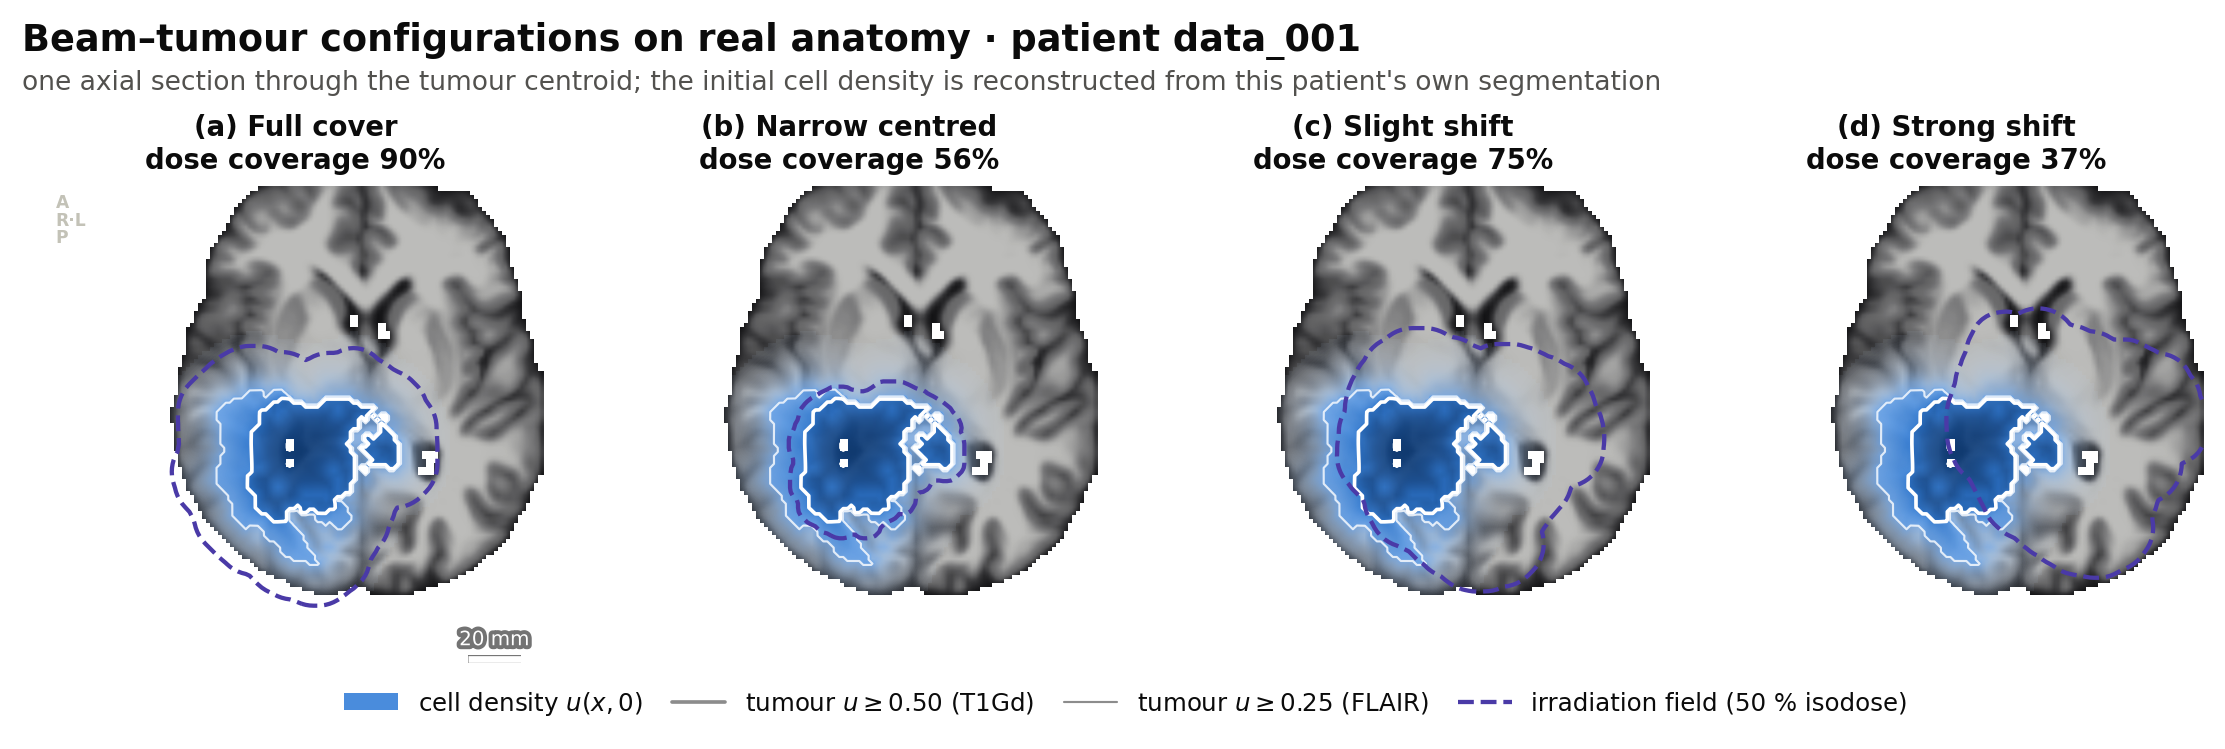
\includegraphics[width=1.0\textwidth]{figures/f3_beam_configs.png}
\caption{The four beam--tumour configurations on one patient's real anatomy.
White contours are the reconstructed tumour iso-surfaces at $u=0.50$ (T1Gd) and
$u=0.25$ (FLAIR); the dashed contour is the 50\,\% isodose. Coverage is the
mass-weighted fraction of tumour inside the field.}
\label{fig:beam_configs}\end{figure}

\begin{figure}[t]\centering
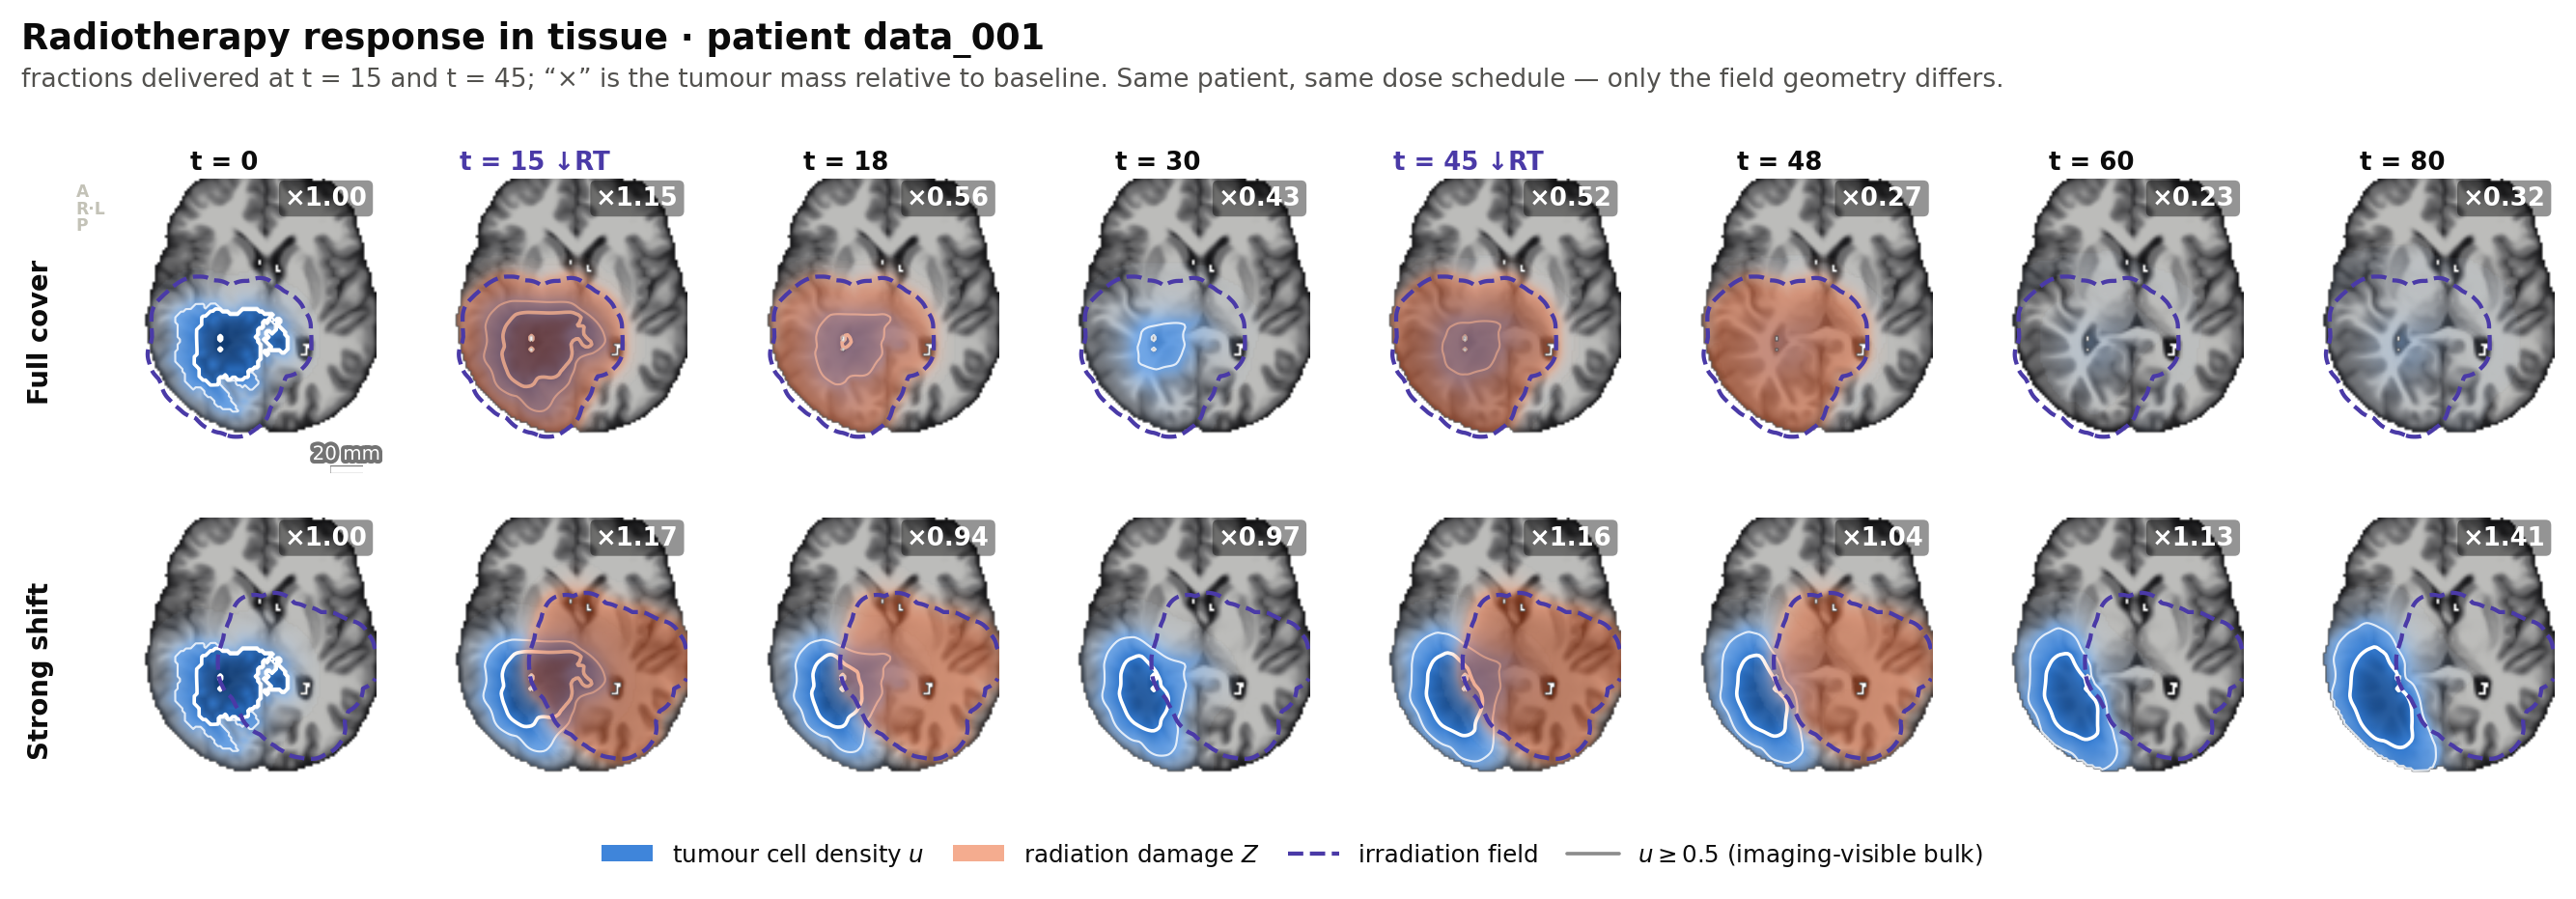
\includegraphics[width=1.0\textwidth]{figures/f4_time_evolution.png}
\caption{Spatial radiotherapy response for one patient: the same dose schedule
under two field geometries. Blue is tumour cell density, orange the
radiation-damage field $Z$, and the annotation is tumour mass relative to
baseline. Under full cover the tumour is driven to a fraction of its initial
mass; under the displaced field the untreated shoulder survives and regrows.}
\label{fig:time_evolution}\end{figure}

\begin{figure}[t]\centering
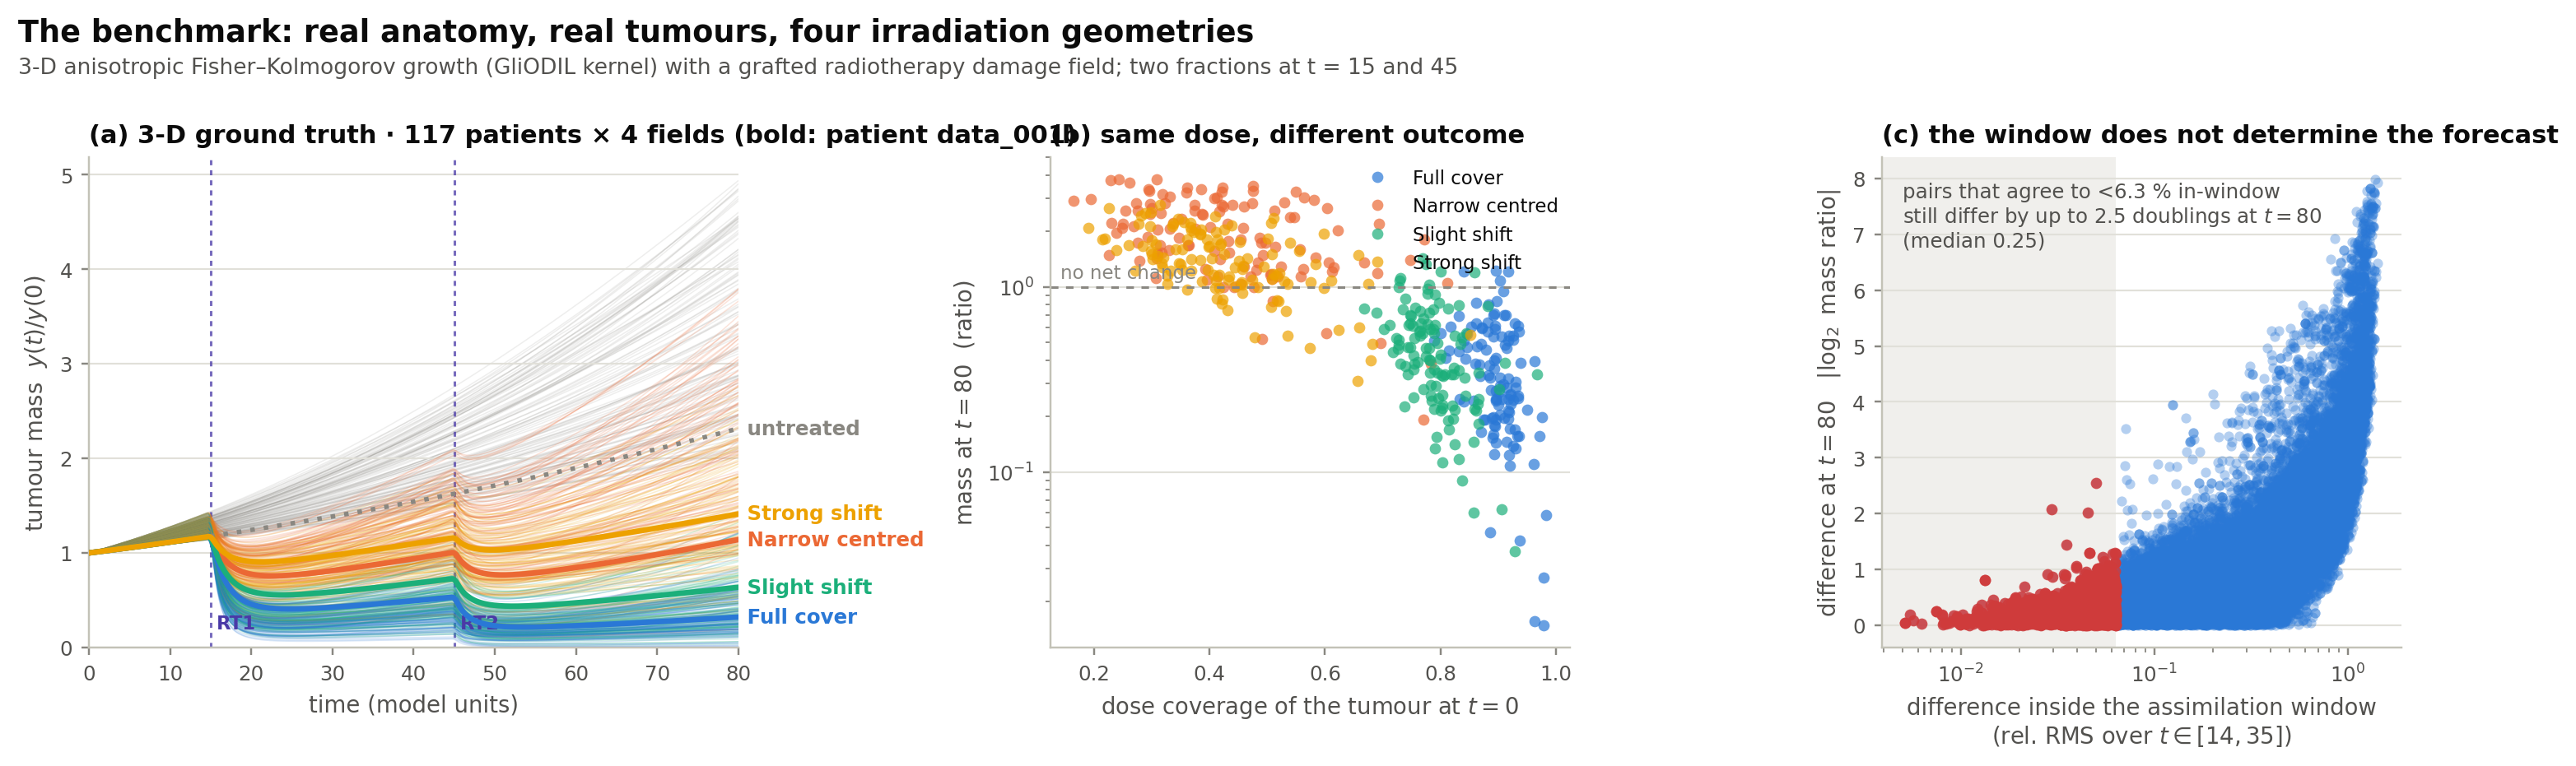
\includegraphics[width=1.0\textwidth]{figures/f1_ground_truth.png}
\caption{(a) Reference mass trajectories for all 117 patients and four
geometries. (b) Delivered dose against outcome. (c) The premise of the study,
quantified: pairs of trajectories that agree closely inside the assimilation
window still diverge by up to several doublings at $t=80$, so the window alone
does not determine the forecast.}
\label{fig:ground_truth}\end{figure}

\subsection{Assimilation Protocol}

For every (patient, configuration) pair we draw $N_{\mathrm{fit}}=20$ evenly
spaced observations on $[14,35]$ --- one time unit earlier than
Table~\ref{tab:assimilation} so that the window brackets the whole first
fraction rather than beginning on it --- perturb them with
$\mathcal{N}\bigl(0,(0.02\,y_i)^2\bigr)$ noise in 20 independent realisations,
and forecast $(35,80]$, which contains the second, unseen irradiation event.
This gives $468$ patient--configuration columns and
$20468$ independently fitted models per method.

All surrogates share one fitting procedure: the same batched fourth-order
Runge--Kutta integrator on a fixed refined grid (decoupled from the observation
times, so a fitted parameter cannot depend on how densely the tumour happened to
be measured), the same optimiser and budget, and the same number of random
restarts. Differences in accuracy are therefore differences between models, not
between fitting procedures.

\paragraph{Compute.}
The unrolled Runge--Kutta loop over a two-state system is kernel-launch bound
rather than compute bound, so batch width is almost free: widening the batch
$22\times$ costs $1.4\times$ the wall-clock. Every method is therefore fitted for
the entire cohort in one tensor whose batch axis carries
(patient $\times$ configuration $\times$ noise realisation $\times$ restart) ---
of order $10^{4}$ independent reduced models trained simultaneously per method.
The reported experiments were run on eight NVIDIA RTX 6000 Ada GPUs, two worker
processes per device.

\subsection{The Growth Law Implied by the Reference Dynamics}

Before comparing surrogates it is worth checking which reduced growth law the
three-dimensional reference actually follows, since this is a property of the
data and not of any surrogate. On the untreated trajectories, $y^{1/3}$ is
linear in $t$ with median $R^{2}=0.9995$, against $0.9864$ for the mass
itself, and the effective exponent recovered from
$\mathrm{d}\log\dot y/\mathrm{d}\log y$ has median $0.81$
($0.65$--$0.90$ over the cohort). This confirms
Eq.~\eqref{eq:volumetric_rate} empirically and locates the truth between the
surface-growth exponent $2/3$ and the logistic exponent $1$, distinctly away
from the latter (Fig.~\ref{fig:growth_law}).

\begin{figure}[t]\centering
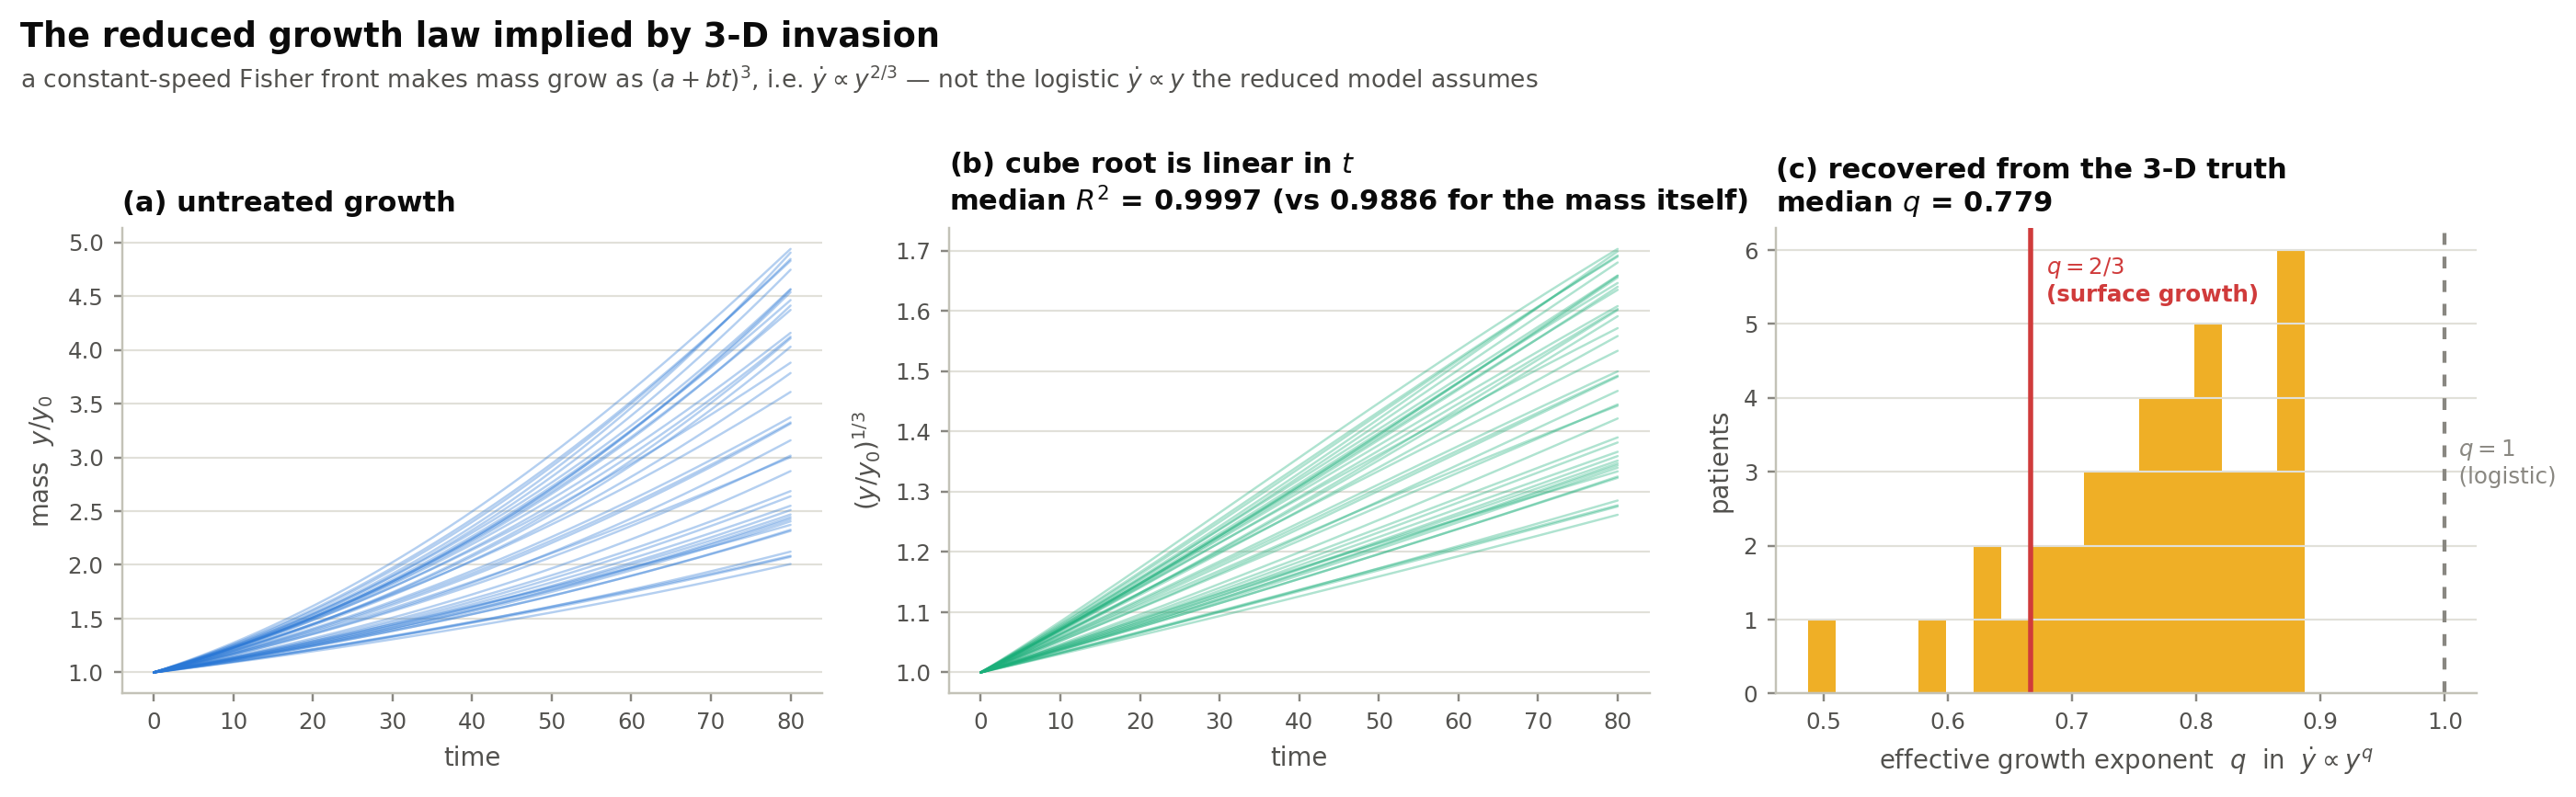
\includegraphics[width=1.0\textwidth]{figures/f2_growth_law.png}
\caption{The reduced growth law implied by three-dimensional invasion.
(a) Untreated reference trajectories. (b) Their cube roots, which are linear in
time. (c) The effective growth exponent $q$ recovered per patient, against the
surface-growth value $2/3$ and the logistic value $1$.}
\label{fig:growth_law}\end{figure}

\subsection{How Much of the Gap Is Structural?}

A forecast error mixes two things: what the reduced model \emph{cannot
represent}, and what it \emph{cannot infer} from twenty noisy samples. We
separate them by fitting each backbone a second time to the entire noise-free
trajectory over $[14,80]$ --- an oracle with no estimation error at all. The
residual of that fit is the irreducible closure gap, and it is exactly the
quantity a learned closure exists to absorb.

% ==========================================================================
% Evaluation on real glioma anatomy -- results
% (continues the section opened in 06-real-data-setup.tex)
% ==========================================================================

\subsection{Surrogate Accuracy}
\label{sec:results_main}

Table~\ref{tab:main_results} reports every surrogate on the same
$468$ patient--configuration columns, Table~\ref{tab:per_case} splits the
same numbers by irradiation geometry, and Fig.~\ref{fig:forecasts} shows the
forecasts for one patient.

\begin{table}[H]
\caption{Forecast accuracy on the real cohort. ``Test'' is the relative RMSE on
$(35,80]$, median over $468$ patient--configuration columns and 20 noisy
assimilation realisations; IQR is its inter-quartile range across columns;
$|e_{80}|$ is the absolute final-time error; ``Train'' is the in-window fit
(the observation noise floor is 2\,\%); $\bar\Phi$ is the realised physics
share of Eq.~\eqref{eq:phi}.}
\label{tab:main_results}
\centering\scriptsize
\setlength{\tabcolsep}{4pt}
%
\begin{tabular}{lrrrrr}
\hline
\textbf{Surrogate} & \textbf{Test} & \textbf{IQR} & $\bm{|e_{80}|}$ & \textbf{Train} & $\bm{\bar\Phi}$ \\
 & (\%) & & (\%) & (\%) & \\
\hline
ODE (logistic, $q{=}1$) & 25.62 & 16.8 & 31.0 & 1.63 & 1.00 \\
ODE (volumetric, $q{=}2/3$) & 23.17 & 13.5 & 25.1 & 1.60 & 1.00 \\
ODE (trained $q$) & 26.05 & 15.4 & 31.2 & 1.57 & 1.00 \\
NODE & 28.49 & 19.0 & 34.7 & 1.32 & 0.00 \\
PI-NODE $(\omega,s_r){=}(0.05,0.10)$ & \textbf{20.78} & \textbf{25.0} & \textbf{24.5} & \textbf{1.73} & \textbf{0.18} \\
PI-NODE $(\omega,s_r){=}(0.20,0.05)$ & 21.87 & 13.2 & 26.2 & 1.44 & 0.36 \\
PI-NODE, volumetric backbone & 21.49 & 14.0 & 26.4 & 1.44 & 0.39 \\
CPI-NODE $\lambda{=}0.4$ & 28.00 & 17.9 & 35.2 & 1.34 & 0.61 \\
CPI-NODE $\lambda{=}0.4$, identified & 24.64 & 13.3 & 29.2 & 1.42 & 0.91 \\
CPI-NODE, identified, trained $q$ & 24.40 & 12.6 & 29.2 & 1.41 & 0.91 \\
GPI-NODE (learned gate) & 24.24 & 13.0 & 26.9 & 1.56 & 0.92 \\
GPI-NODE, identified & 23.77 & 12.8 & 26.9 & 1.47 & 1.00 \\
GPI-NODE, identified + autonomous & 23.77 & 12.8 & 27.1 & 1.46 & 1.00 \\
Bounded closure only ($\lambda{=}1$) & 26.05 & 90.7 & 20.5 & 21.29 & 0.00 \\
Bounded closure only, autonomous & 30.21 & 78.6 & 40.8 & 21.30 & 0.00 \\
\hline
\end{tabular}

\end{table}

\begin{table}[H]
\caption{Forecast relative RMSE (\%) by irradiation geometry; median over
patients and realisations. The best entry in each column is bold.}
\label{tab:per_case}
\centering\scriptsize
\setlength{\tabcolsep}{5pt}
%
\begin{tabular}{lrrrr}
\hline
\textbf{Surrogate} & \textbf{Full} & \textbf{Narrow} & \textbf{Slight} & \textbf{Strong} \\
\hline
ODE (logistic, $q{=}1$) & 38.1 & 25.9 & 29.7 & 18.9 \\
ODE (volumetric, $q{=}2/3$) & \textbf{29.8} & 27.0 & 21.8 & 20.0 \\
ODE (trained $q$) & 35.6 & 27.1 & 28.3 & 19.9 \\
NODE & 47.4 & 29.4 & 32.1 & 21.8 \\
PI-NODE $(\omega,s_r){=}(0.05,0.10)$ & 39.0 & 14.2 & 36.9 & 12.3 \\
PI-NODE $(\omega,s_r){=}(0.20,0.05)$ & 32.9 & 20.1 & 22.9 & 18.2 \\
PI-NODE, volumetric backbone & 34.5 & 20.4 & 23.3 & 17.5 \\
CPI-NODE $\lambda{=}0.4$ & 40.4 & 26.6 & 30.6 & 20.9 \\
CPI-NODE $\lambda{=}0.4$, identified & 34.2 & 26.0 & 24.1 & 21.1 \\
CPI-NODE, identified, trained $q$ & 34.1 & 25.1 & 24.1 & 20.4 \\
GPI-NODE (learned gate) & 31.3 & 26.4 & 22.7 & 21.2 \\
GPI-NODE, identified & 30.0 & 27.2 & 20.5 & 21.3 \\
GPI-NODE, identified + autonomous & 30.0 & 27.0 & \textbf{20.4} & 21.3 \\
Bounded closure only ($\lambda{=}1$) & 100.0 & \textbf{9.8} & 70.2 & \textbf{9.1} \\
Bounded closure only, autonomous & 100.0 & 31.8 & 29.2 & 23.8 \\
\hline
\end{tabular}

\end{table}

\begin{figure}[t]\centering
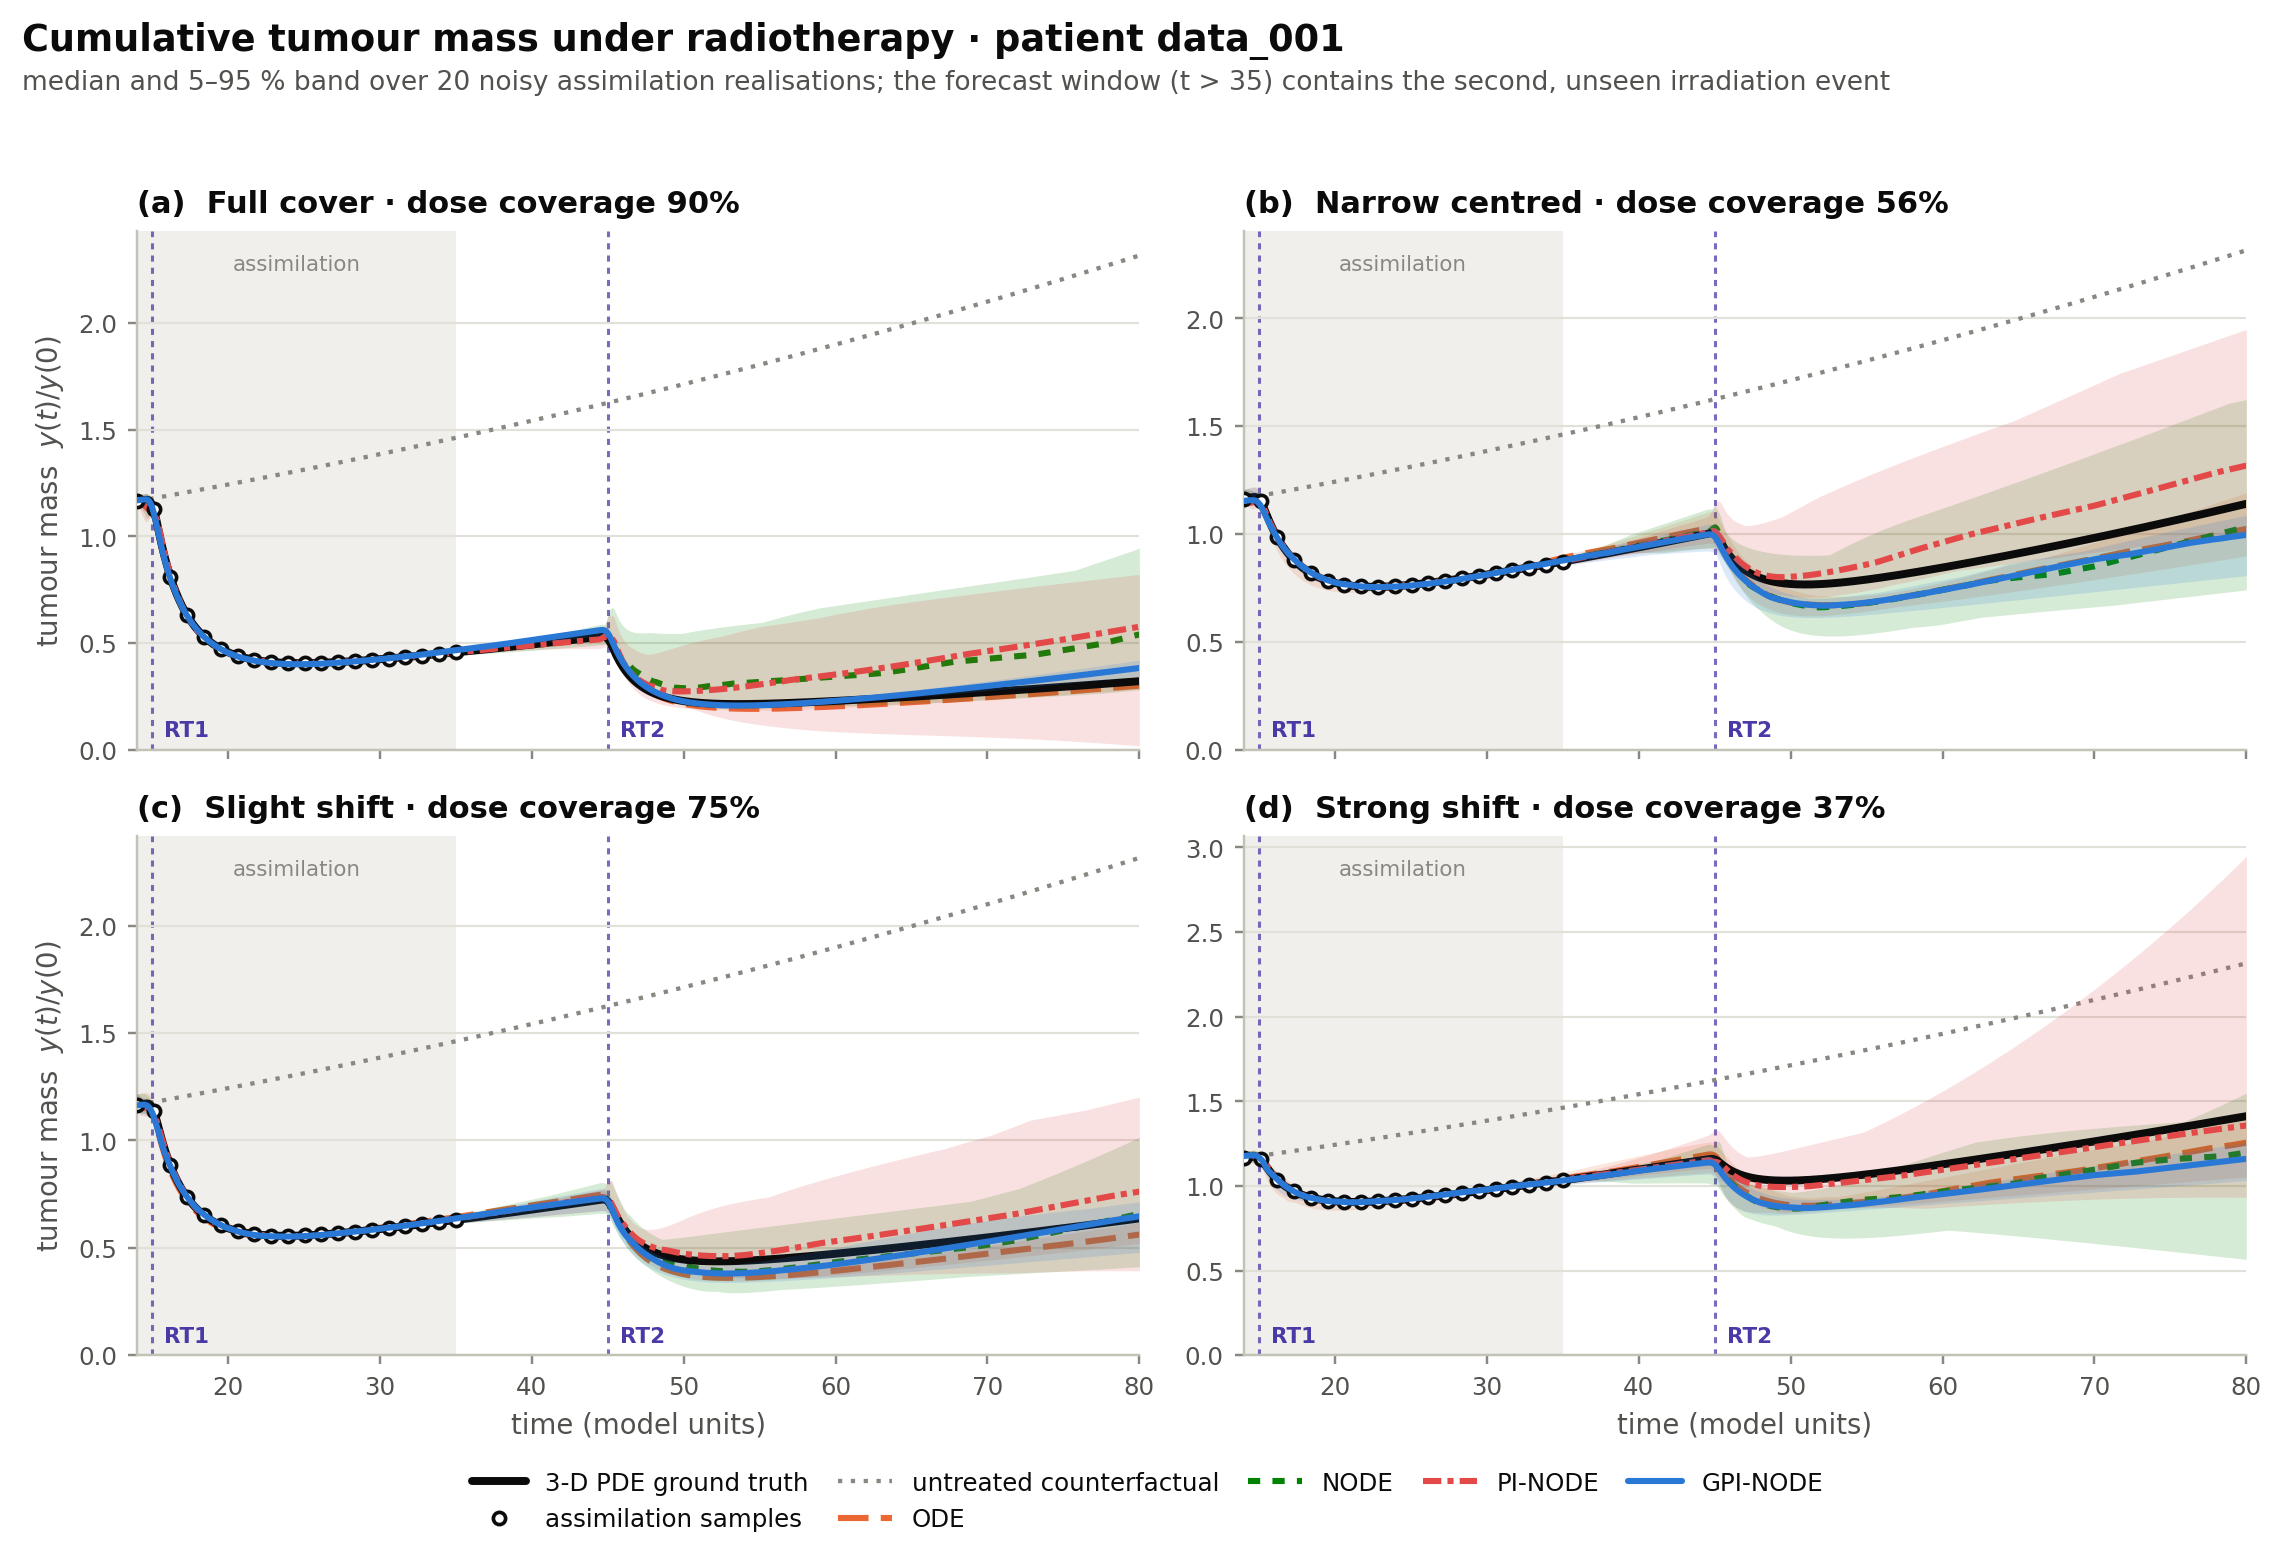
\includegraphics[width=1.0\textwidth]{figures/f5_forecasts.png}
\caption{Cumulative tumour mass for one patient under the four irradiation
geometries. Black is the three-dimensional reference, circles the sparse noisy
observations used for assimilation, and the bands are the 5--95\,\% range over
20 noisy realisations. The forecast window contains the second, unseen
fraction. Every model reproduces the assimilation window; they separate only
after it.}
\label{fig:forecasts}\end{figure}

\paragraph{The paper's central claim is confirmed, and by a wider margin than on
the phantom.} On the two geometry-mismatched configurations --- the situations
this work is about --- a learned closure is decisively better than any purely
mechanistic surrogate: on \texttt{narrow\_centered} the best mechanistic model
reaches 25.9\,\% against 9.8\,\% for a
bounded learned closure, and on \texttt{strong\_shift}
18.9\,\% against 9.1\,\%. That is a factor of
$2$--$3$, on real anatomy, for exactly the effect the closure was introduced to
capture.

\paragraph{The optimum inverts with the geometry.} Where the field covers the
tumour the purely mechanistic model wins and an unconstrained closure fails
outright; where the field is under-sized or displaced the ordering reverses
(Table~\ref{tab:per_case}). The realised physics share of the per-configuration
winner runs from $\Phi\approx1$ to $\Phi\approx0$ within the same cohort. For a
\emph{bounded} closure this makes a single $\lambda$ costly --- forcing one
value everywhere costs up to 148\,\% on the worst
configuration --- which is the argument for the state-dependent gate of
Eq.~\eqref{eq:gate}. For the \emph{unbounded} closure of
Eq.~\eqref{eq:pinode_weighted} a single setting suffices
(8\,\%), precisely because an unbounded closure is
free to adapt itself per patient without help from the weight. Bounding it buys
identifiability and costs that adaptivity.

\paragraph{PI-NODE's overall advantage is not statistically resolved, and it is
the least reliable model.} Its median is the lowest
(20.78\,\%), but a paired Wilcoxon test over the $468$ columns
--- every method sees the same columns and the same noise --- does not separate
it from the volumetric mechanistic model, from its own retuned variant, or from
the gated form proposed here ($p$ between $0.4$ and $0.7$). It also carries by
far the widest spread across the cohort, visible directly as the broad band in
Fig.~\ref{fig:forecasts}. The gated, identified form matches it within noise at
roughly half the inter-quartile range, and reports a calibrated $\lambda$ where
$(\omega,s_{r})$ reports nothing. The honest claim for the replacement is
therefore identifiability and reliability at no significant accuracy cost, not
an accuracy win.

\paragraph{Most of the error is estimation, not model inadequacy.}
Fitting each backbone to the entire noise-free trajectory leaves an irreducible
residual of only 6.96\,\% (logistic) and 6.79\,\%
(volumetric); the assimilated models score several times that
(Fig.~\ref{fig:error_budget}). The dominant limitation is not that the reduced
form cannot represent the dynamics --- it is that twenty noisy samples over a
short window do not determine its parameters. This reframes what a closure term
must achieve: added flexibility has to buy more than the estimation variance it
costs, which is why an unconstrained correction of \emph{small} magnitude is the
most damaging configuration of all --- free enough to absorb in-window noise,
and compounding across the forecast.

\begin{figure}[t]\centering
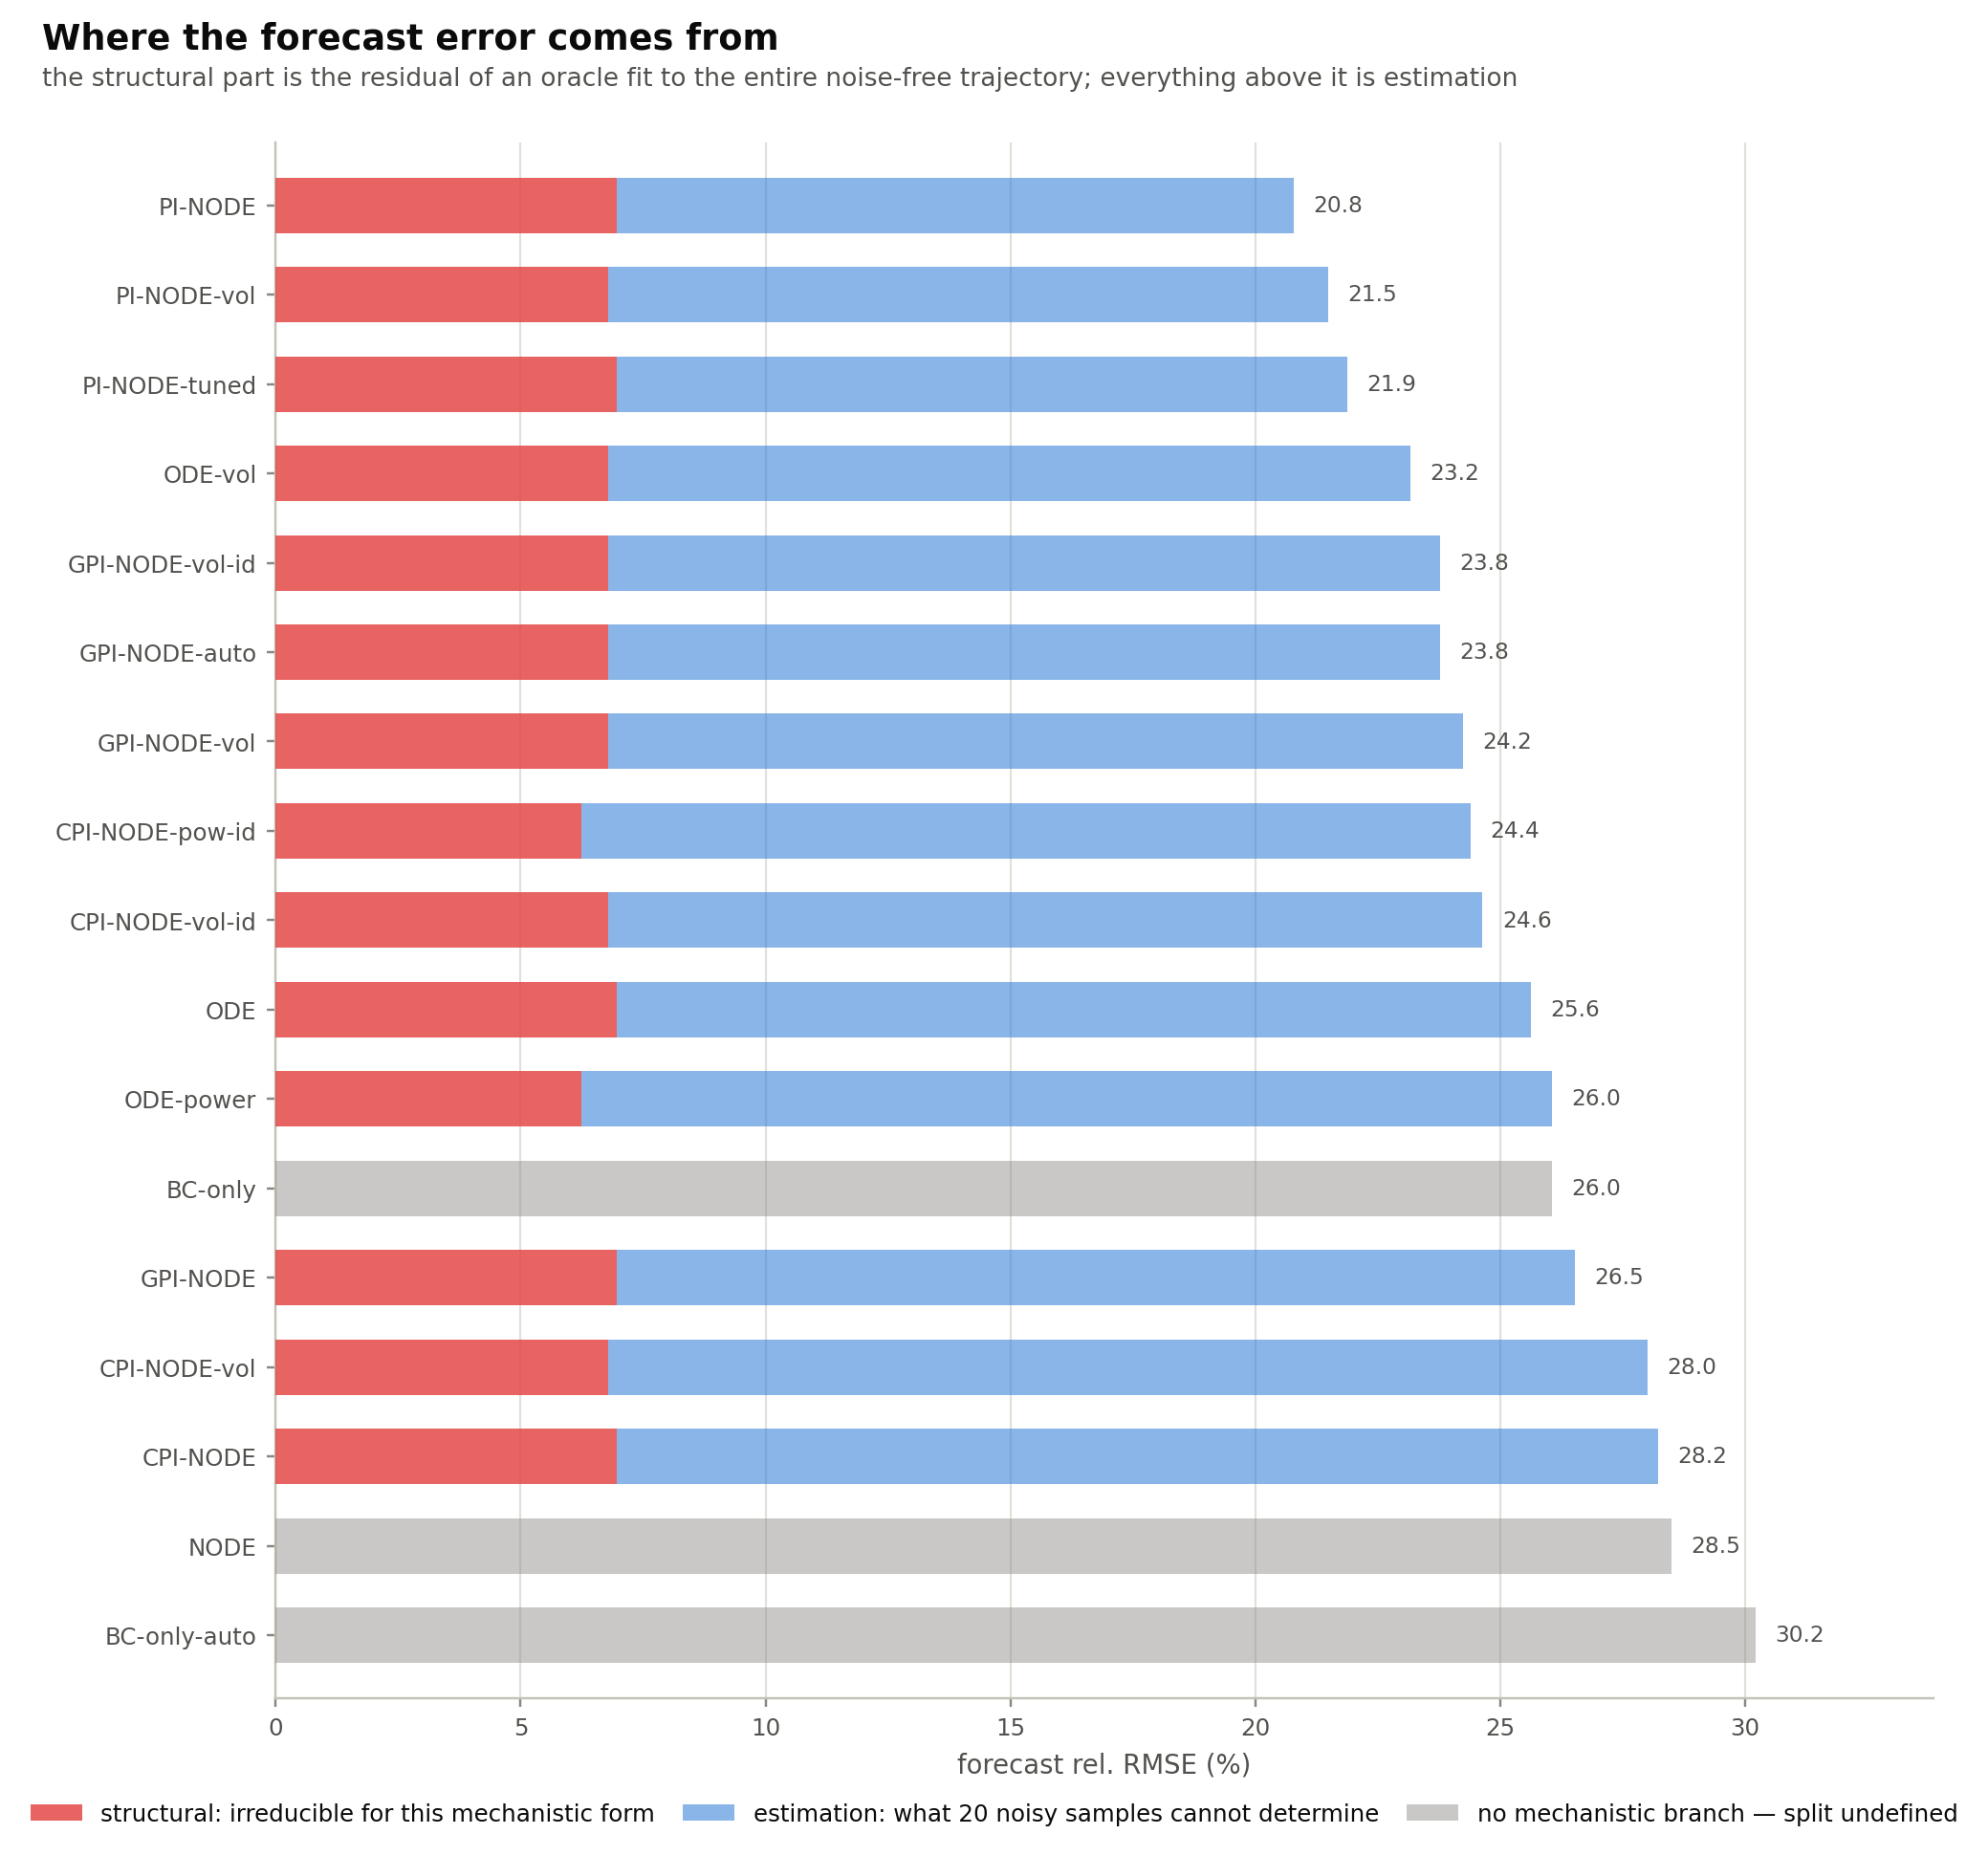
\includegraphics[width=0.95\textwidth]{figures/f9_error_budget.png}
\caption{Decomposition of the forecast error. The structural part is the
residual of an oracle fit to the entire noise-free trajectory --- the best the
model form can do with no estimation error at all; everything above it is what
sparse noisy assimilation fails to determine.}
\label{fig:error_budget}\end{figure}

\begin{figure}[t]\centering
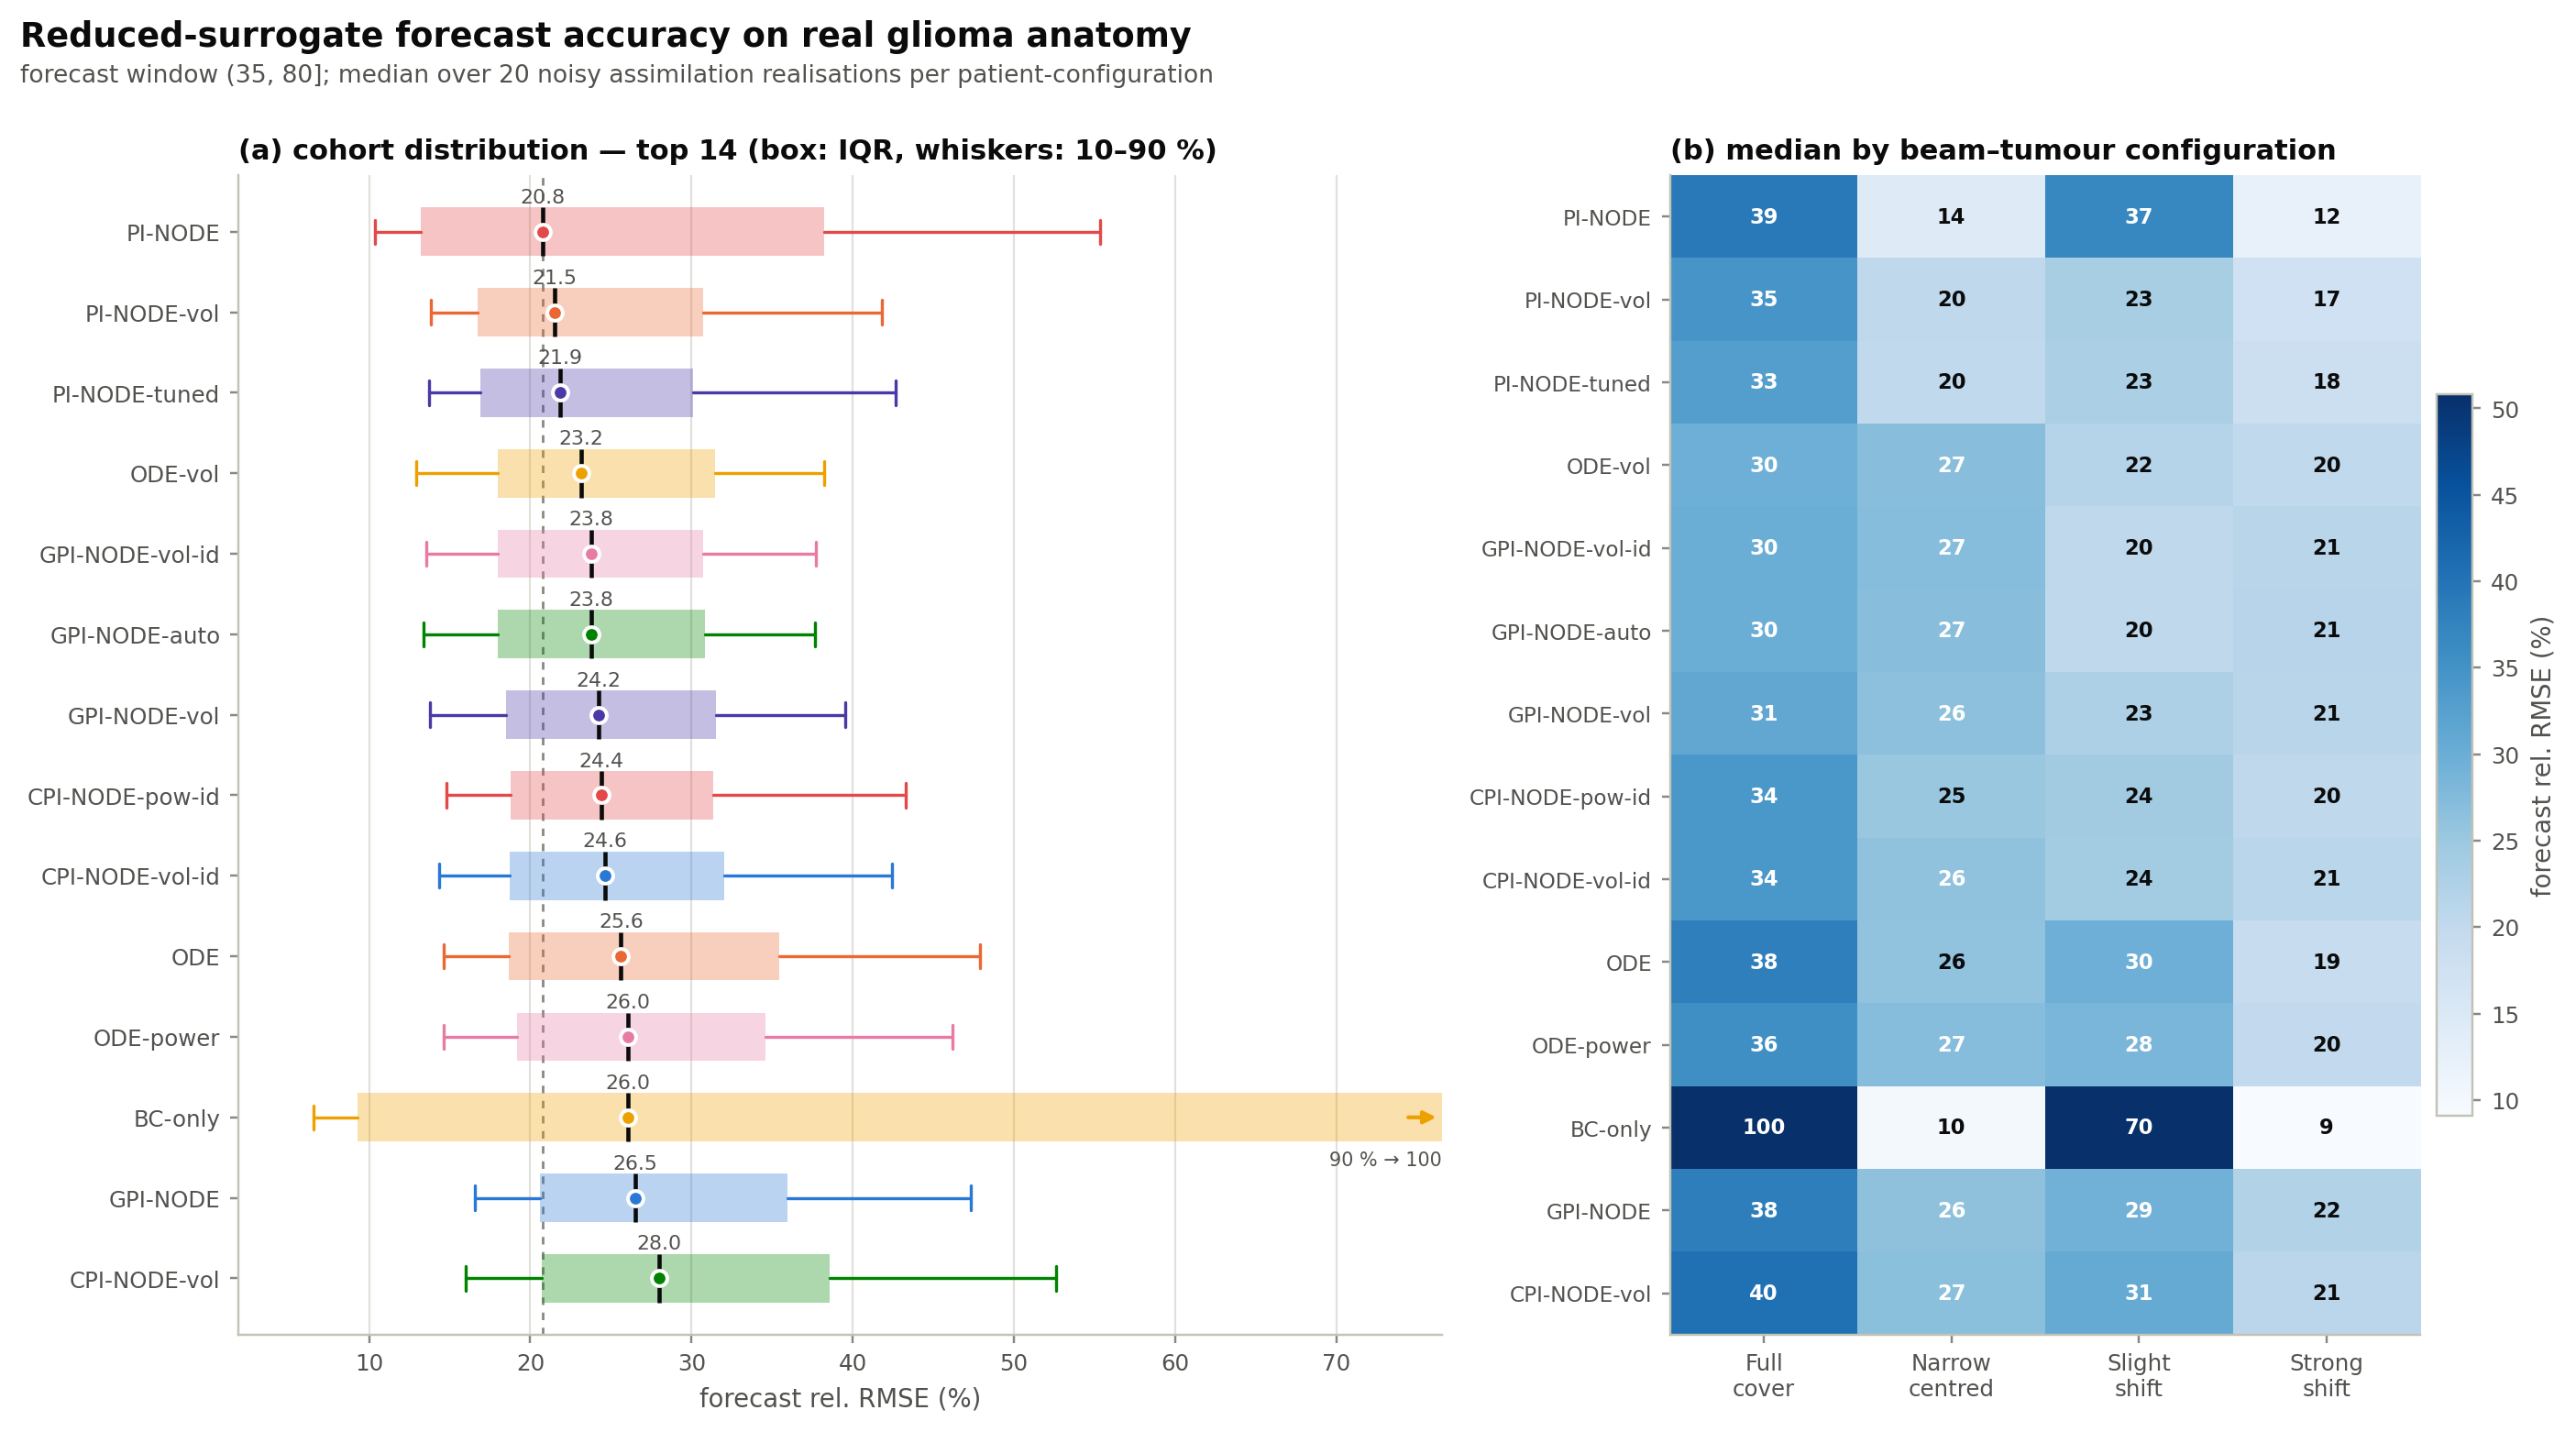
\includegraphics[width=1.0\textwidth]{figures/f8_cohort_accuracy.png}
\caption{Cohort distribution of the forecast error per surrogate, and its median
per irradiation geometry.}
\label{fig:cohort_accuracy}\end{figure}

\subsection{Is the Physics--Closure Weight a Real Control?}
\label{sec:results_weights}

Section~\ref{sec:gauge} shows $(\omega,s_r)$ cannot be normalised. This section
asks the operational question instead: does the nominal weight predict the
balance the fitted model actually adopts? We sweep both parameterisations on the
same backbone and compare the nominal machine-learning share ---
$s_r/(\omega+s_r)$ for Eq.~\eqref{eq:pinode_weighted}, $\lambda$ for
Eq.~\eqref{eq:cpinode} --- against the realised share $1-\bar\Phi$ of
Eq.~\eqref{eq:phi}.

\begin{table}[H]
\caption{Nominal versus realised machine-learning share. $|\Delta|$ is the
calibration error.}
\label{tab:weights}
\centering\scriptsize
\setlength{\tabcolsep}{4pt}
%
\begin{tabular}{llrrrr}
\hline
\textbf{Parameterisation} & \textbf{Setting} & \textbf{nominal} & \textbf{realised} & $\bm{|\Delta|}$ & \textbf{Test (\%)} \\
\hline
$\omega f_{RT}+s_r g_\psi$ & $\omega{=}$1, $s_r{=}$0.02 & 0.020 & 0.459 & 0.439 & 37.31 \\
 & $\omega{=}$0.5, $s_r{=}$0.02 & 0.038 & 0.413 & 0.374 & 25.20 \\
 & $\omega{=}$1, $s_r{=}$0.05 & 0.048 & 0.475 & 0.427 & 37.73 \\
 & $\omega{=}$0.2, $s_r{=}$0.02 & 0.091 & 0.609 & 0.518 & 20.13 \\
 & $\omega{=}$0.5, $s_r{=}$0.05 & 0.091 & 0.461 & 0.370 & 27.88 \\
 & $\omega{=}$1, $s_r{=}$0.1 & 0.091 & 0.483 & 0.392 & 37.02 \\
 & $\omega{=}$0.5, $s_r{=}$0.1 & 0.167 & 0.480 & 0.314 & 29.02 \\
 & $\omega{=}$1, $s_r{=}$0.2 & 0.167 & 0.489 & 0.322 & 37.07 \\
 & $\omega{=}$0.2, $s_r{=}$0.05 & 0.200 & 0.623 & 0.423 & 21.49 \\
 & $\omega{=}$0.05, $s_r{=}$0.02 & 0.286 & 0.821 & 0.535 & 15.09 \\
 & $\omega{=}$0.5, $s_r{=}$0.2 & 0.286 & 0.494 & 0.208 & 28.45 \\
 & $\omega{=}$0.2, $s_r{=}$0.1 & 0.333 & 0.628 & 0.294 & 23.50 \\
 & $\omega{=}$0.02, $s_r{=}$0.02 & 0.500 & 0.900 & 0.400 & 14.47 \\
 & $\omega{=}$0.05, $s_r{=}$0.05 & 0.500 & 0.816 & 0.316 & 18.96 \\
 & $\omega{=}$0.2, $s_r{=}$0.2 & 0.500 & 0.630 & 0.130 & 23.60 \\
 & $\omega{=}$0.05, $s_r{=}$0.1 & 0.667 & 0.814 & 0.148 & 21.38 \\
 & $\omega{=}$0.02, $s_r{=}$0.05 & 0.714 & 0.897 & 0.183 & 18.65 \\
 & $\omega{=}$0.05, $s_r{=}$0.2 & 0.800 & 0.814 & 0.014 & 23.10 \\
 & $\omega{=}$0.02, $s_r{=}$0.1 & 0.833 & 0.896 & 0.063 & 22.19 \\
 & $\omega{=}$0.02, $s_r{=}$0.2 & 0.909 & 0.899 & 0.010 & 25.45 \\
\hline
$(1{-}\lambda)f_{RT}+\lambda\sigma\tanh g_\psi$ & $\lambda{=}$0 & 0.000 & 0.000 & 0.000 & 23.17 \\
 & $\lambda{=}$0.1 & 0.100 & 0.355 & 0.255 & 28.67 \\
 & $\lambda{=}$0.2 & 0.200 & 0.418 & 0.218 & 29.80 \\
 & $\lambda{=}$0.2 & 0.200 & 0.398 & 0.198 & 29.25 \\
 & $\lambda{=}$0.3 & 0.300 & 0.424 & 0.124 & 29.41 \\
 & $\lambda{=}$0.4 & 0.400 & 0.412 & 0.012 & 28.00 \\
 & $\lambda{=}$0.4 & 0.400 & 0.384 & 0.016 & 26.29 \\
 & $\lambda{=}$0.5 & 0.500 & 0.413 & 0.087 & 25.71 \\
 & $\lambda{=}$0.6 & 0.600 & 0.445 & 0.155 & 24.06 \\
 & $\lambda{=}$0.6 & 0.600 & 0.427 & 0.173 & 23.36 \\
 & $\lambda{=}$0.7 & 0.700 & 0.519 & 0.181 & 22.95 \\
 & $\lambda{=}$0.8 & 0.800 & 0.615 & 0.185 & 21.58 \\
 & $\lambda{=}$0.8 & 0.800 & 0.600 & 0.200 & 23.39 \\
 & $\lambda{=}$0.9 & 0.900 & 0.726 & 0.174 & 20.19 \\
 & $\lambda{=}$1 & 1.000 & 1.000 & 0.000 & 26.05 \\
 & $\lambda{=}$1 & 1.000 & 1.000 & 0.000 & 30.21 \\
\hline
\end{tabular}

\end{table}

Both parameterisations are monotone --- a larger nominal share does produce a
larger realised share (Spearman +0.89 and +0.94 respectively)
--- so both are usable as a dial. They differ in whether the dial is
\emph{calibrated}: the mean calibration error is 0.294 for
$(\omega,s_r)$ against 0.124 for $\lambda$, a factor of
2.4. Under Eq.~\eqref{eq:pinode_weighted} a setting whose nominal
machine-learning contribution is a few per cent can realise nearly half the
vector field, and settings whose nominal shares differ several-fold can land on
the same realised balance. Under Eq.~\eqref{eq:cpinode} the number on the dial
is, to within a few per cent, the share the model adopts, and the two endpoints
are exact --- $\lambda=0$ reproduces the assimilated mechanistic model to the
last digit even with a fully trained closure present (verified at
$0$).

\paragraph{Two consequences that are not merely about labelling.}
First, the published default is not the best cell of its own grid: sweeping
$(\omega,s_{r})$ finds $\omega{=}$0.02, $s_r{=}$0.02 at 14.47\,\% against
20.78\,\% for $(0.05,0.10)$, a \emph{32\,\% relative} improvement from
tuning alone. Second, and more informative, the winning cell has a realised
machine-learning share of 0.90: accuracy improves monotonically as
the realised physics share falls, so on this benchmark the formulation works
best as a lightly-anchored neural ODE rather than as a balanced hybrid. It is
worth stating plainly what the published numbers mean --- $(\omega,s_r) =
(0.05,0.10)$ reads as ``5\,\% physics, 10\,\% residual'' and is in fact
$81\,\%$ machine learning.

\paragraph{The original parameterisation cannot reach a physics-dominated
model.} Across the whole $5\times4$ grid the realised machine-learning share
spans only 0.41--0.90 (range 0.49), never
approaching either endpoint; the convex control spans the full
0.00--1.00. This is an expressiveness limitation, not
just an interpretability one: no choice of $(\omega,s_{r})$ in this range yields
the mechanistic model, even though $s_{r}=0$ nominally should.

\begin{figure}[t]\centering
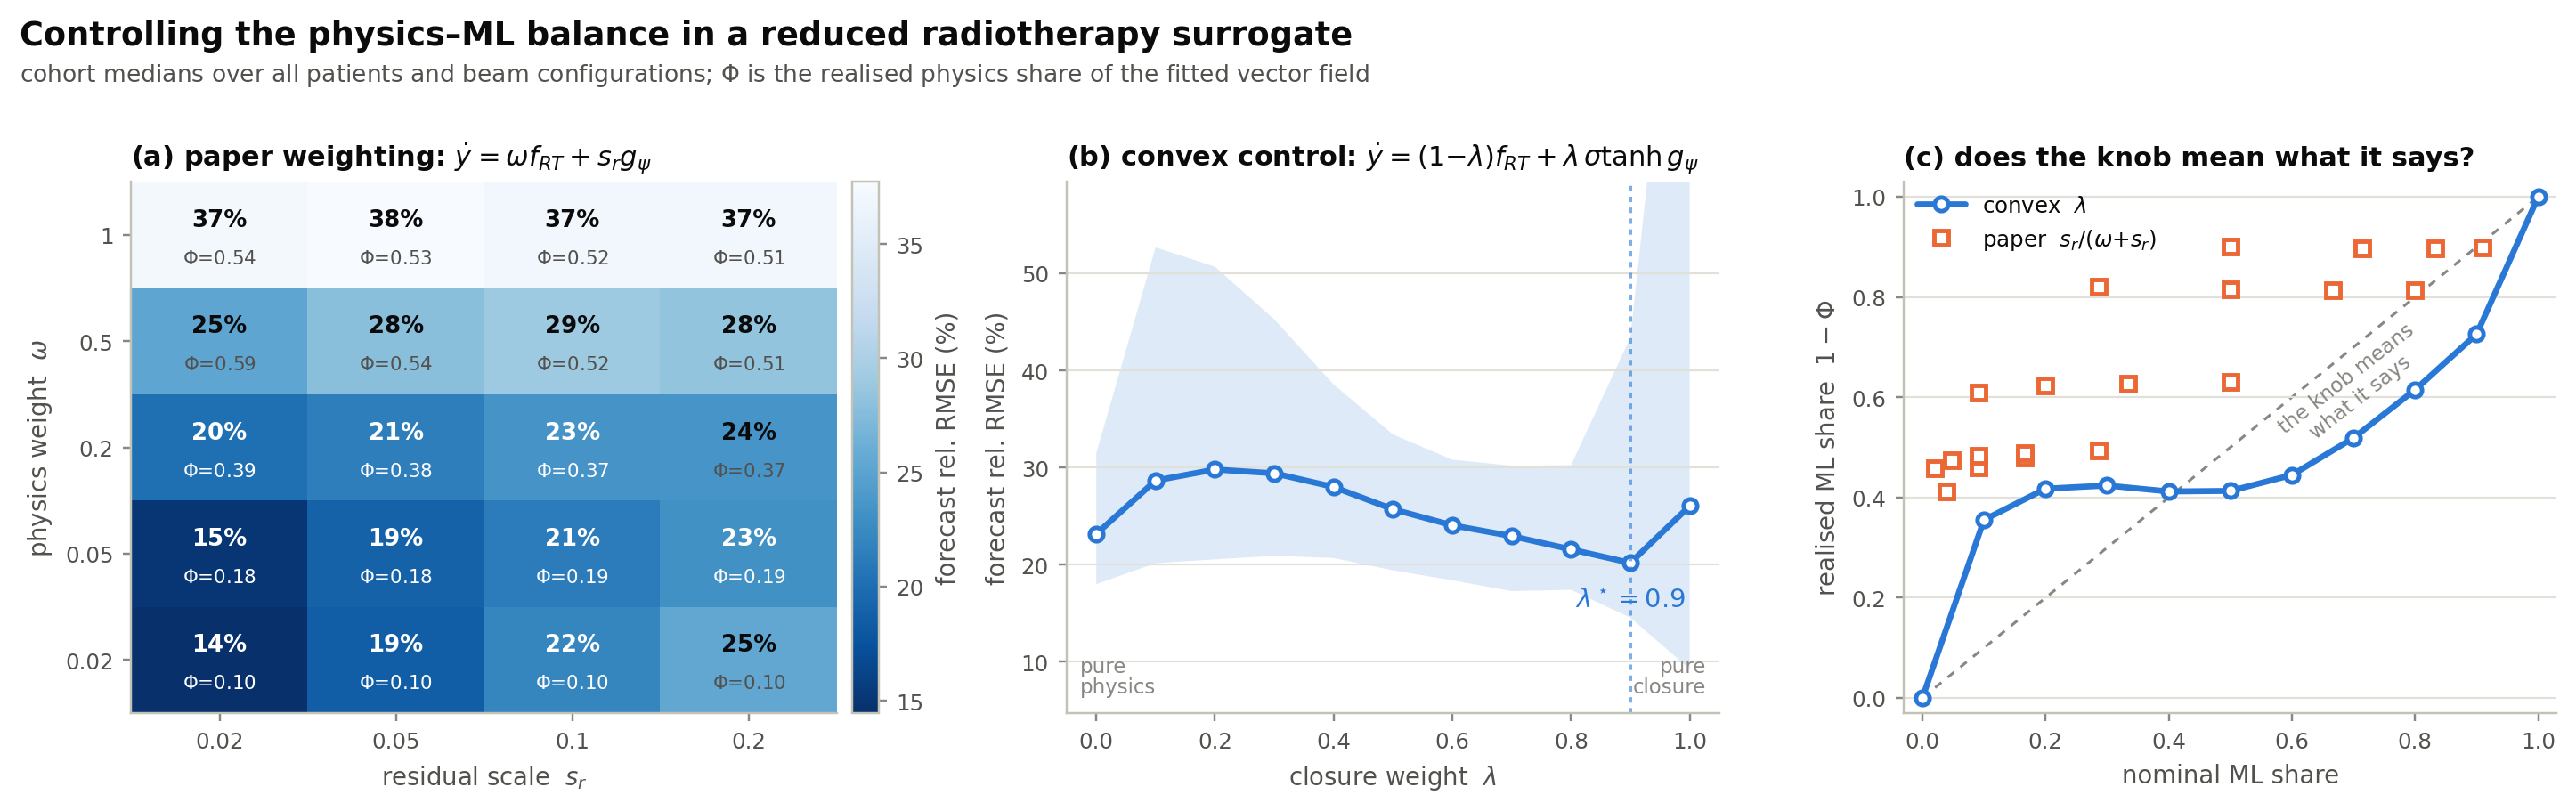
\includegraphics[width=1.0\textwidth]{figures/f6_weight_control.png}
\caption{(a) Forecast error over the $(\omega,s_r)$ grid of
Eq.~\eqref{eq:pinode_weighted}, with the realised physics share $\Phi$ printed
in each cell. (b) The same sweep for the single convex control $\lambda$ of
Eq.~\eqref{eq:cpinode}. (c) Realised against nominal machine-learning share for
both; the diagonal is perfect calibration.}
\label{fig:weight_control}\end{figure}

This is the practical answer to the question the two weights raise. They cannot
be made to sum to one, because both branches are cones and any normalisation is
undone by the branch's own parameters. Replacing them by a bounded closure, an
anchored backbone and an orthogonality constraint restores a single coefficient
that behaves like an interpolation weight, admits classical linear interpolation
between the mechanistic and learned models, and --- unlike $(\omega,s_r)$ ---
can be reported and compared across studies. Given
Section~\ref{sec:results_main}, the coefficient that matters is not a global
constant but the gate of Eq.~\eqref{eq:gate}; the value of making it
identifiable is that its output is then a meaningful readout of \emph{where}
the reduced physics is failing.

\subsection{Can a Learned Gate Recover the Regime-Dependent Optimum?}
\label{sec:results_gate}

Section~\ref{sec:results_main} shows the optimal balance inverts with the
irradiation geometry, and Eq.~\eqref{eq:gate} is the natural response: let
$\lambda$ depend on the state and discover the schedule. Table~\ref{tab:gate}
tests it by varying how strongly the gate is restrained.

\begin{table}[H]
\caption{Gate ablation. $\eta$ is the penalty on the trajectory-averaged gate;
the identifiability rows use $\eta = 0.02$ and add the anchor and orthogonality
terms of Section~\ref{sec:convex} singly and together.}
\label{tab:gate}
\centering\scriptsize
\setlength{\tabcolsep}{5pt}
\begin{tabular}{lrrr}
\hline
\textbf{Variant} & \textbf{Test (\%)} & \textbf{IQR} & $\bm{\bar\Phi}$ \\
\hline
orthogonality only & \textbf{23.5} & 12.2 & 0.97 \\
gate penalty $\eta = 0.3$ & 23.7 & 12.8 & 0.99 \\
anchor + orthogonality + warm start & 23.8 & 12.8 & 1.00 \\
anchor only & 23.9 & 12.9 & 0.97 \\
$\eta = 0.08$ & 24.0 & 13.0 & 0.98 \\
no identifiability terms ($\eta = 0.02$) & 24.2 & 13.0 & 0.93 \\
$\eta = 0.005$ & 27.4 & 14.5 & 0.78 \\
$\eta = 0$ (free gate) & 29.0 & 28.8 & 0.67 \\
\hline
\end{tabular}
\end{table}

The relationship is monotone, and it runs against the hypothesis: \emph{the more
authority the gate takes, the worse the forecast.} A completely free gate settles
at $\bar\Phi\approx0.67$ \emph{uniformly} --- the damaging interior regime ---
and posts the worst result in the group, with three times the spread of the
restrained variants and $52\,\%$ error on the covered configurations.

\paragraph{The natural diagnosis is observability, and it is wrong.}
The reduced state $(y,z,t,U)$ cannot distinguish an under-sized field from a
displaced one, so an obvious explanation is that the gate has no way to know
which regime it is in. We tested this directly by giving the gate the one scalar
that does separate them --- the mass-weighted dose coverage at $t=0$, which any
treatment plan reports without additional measurement. The closure never
receives it, so identifiability is unaffected. The result is a null
(Table~\ref{tab:context}): with and without the signal the forecast error agrees
to within $0.24$ percentage points and the realised shares are identical to two
decimals. The gate ignores the information.

\begin{table}[H]
\caption{Handing the gate an explicit regime signal (dose coverage at $t=0$)
changes nothing. Forecast relative RMSE (\%), full cohort.}
\label{tab:context}
\centering\scriptsize
\setlength{\tabcolsep}{6pt}
\begin{tabular}{rrrr}
\hline
$\bm{\eta}$ & \textbf{gate with coverage} & \textbf{gate without} & $\bm{\Delta}$ \\
\hline
0 & 28.42 & 28.45 & $-0.03$ \\
0.005 & 27.02 & 27.02 & $0.00$ \\
0.02 & 23.73 & 23.80 & $-0.07$ \\
0.08 & \textbf{23.12} & 23.36 & $-0.24$ \\
\hline
\end{tabular}
\end{table}

\paragraph{The schedule has no in-window signature.}
The explanation is in the training column of Table~\ref{tab:gate}: it is flat at
$1.3$--$1.6\,\%$ --- the observation-noise floor --- while the forecast error
moves from $29.0\,\%$ to $23.7\,\%$. Every setting of the gate fits the
assimilation window equally well. The regime distinction pays only in the
forecast window, which the objective never sees, so no gate can learn a
forecast-improving schedule from an in-window loss, however it is parameterised
and whatever side information it is given. The gate does not lack information;
it lacks a reason to use it. The penalty $\eta$ helps monotonically precisely
because it substitutes an explicit prior for a signal the loss cannot supply.

This sharpens the ambiguity measured in Fig.~\ref{fig:ground_truth}(c). That
window-indistinguishable trajectories diverge afterwards is not only why a
closure term is needed --- it is why the closure's schedule cannot be fitted.

The same tables correct a natural mis-attribution. Within the gated family the
identifiability terms \emph{improve} accuracy --- $24.2\,\%$ without them,
$23.5\,\%$ with the orthogonality projection alone. The accuracy cost identified
in Section~\ref{sec:results_weights} is not the anchor or the projection; it is
the $\tanh$ \emph{bound}, which is precisely the ingredient that removes the
$s_{r}$ gauge.

\paragraph{Consequence: set the balance, do not learn it.} The physics--closure
balance is a plan-time decision. The treatment geometry is known before any
response data exists, the right choice is worth a factor of two to three
(Section~\ref{sec:results_main}), and a conformal well-covering field calls for
a physics-dominated surrogate while an under-sized or displaced one calls for
closure authority. Learning the schedule instead would require an objective that
can see the payoff --- a forecast-window loss, and therefore a longitudinal
cohort with a post-treatment observation. That is a data-collection requirement,
not a modelling one.

\begin{figure}[t]\centering
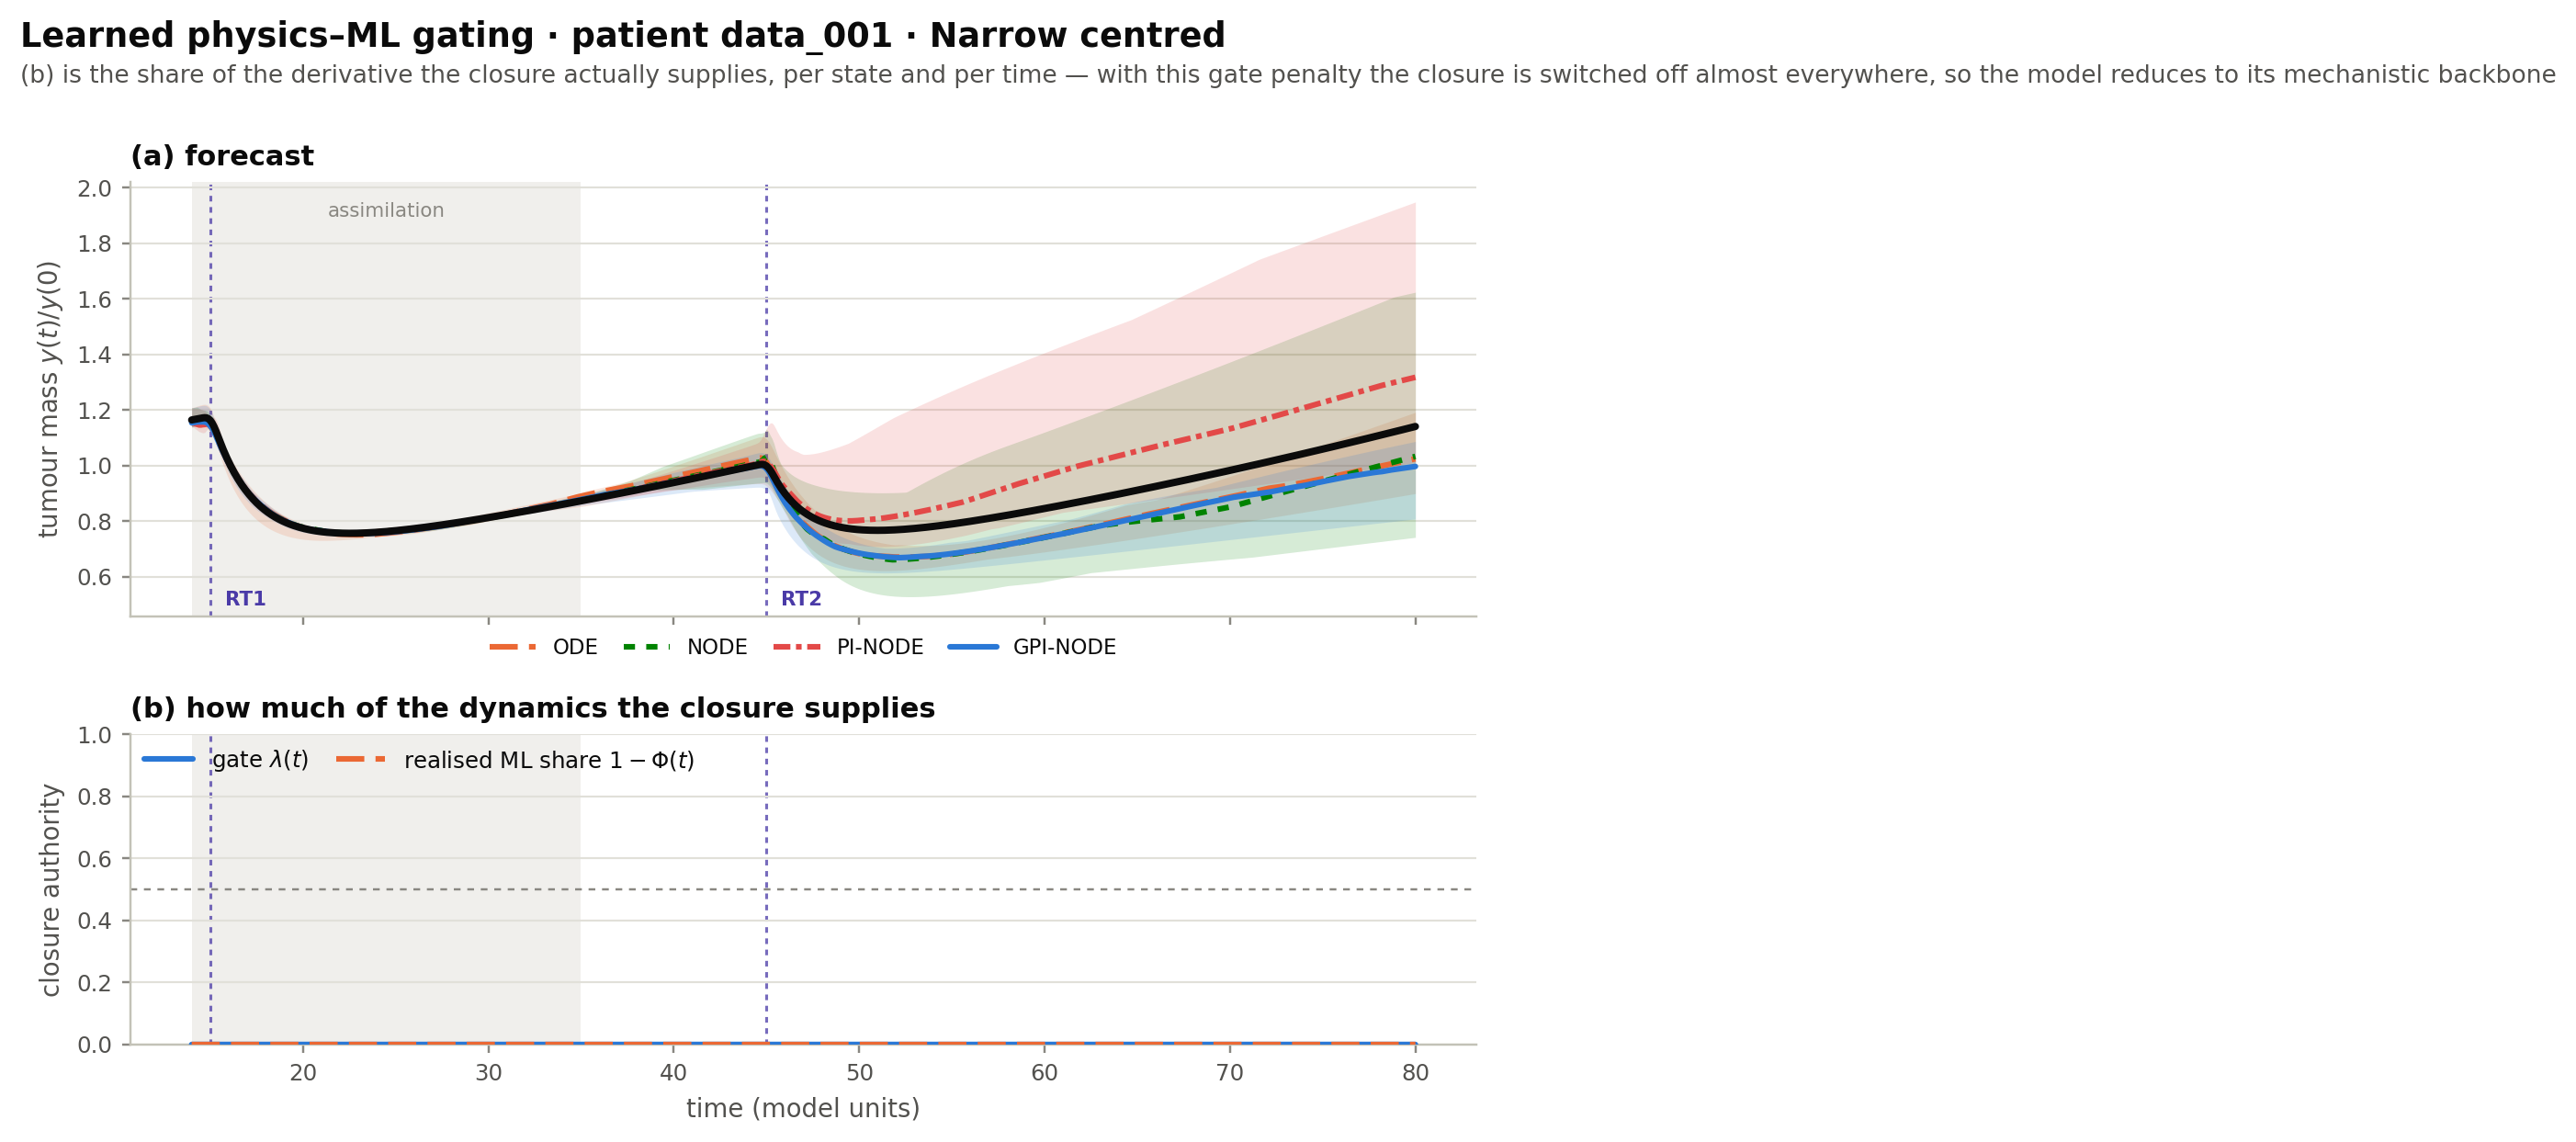
\includegraphics[width=0.85\textwidth]{figures/f7_gate.png}
\caption{The learned gate of Eq.~\eqref{eq:gate}: the forecast, and the share of
the derivative the closure actually supplies as a function of time. At the gate
penalty used here the closure is switched off almost everywhere and the model
reduces to its mechanistic backbone --- a faithful readout of what the fit
chose, and the reason the identified variant forfeits the closure advantage
available on the mismatched geometries.}
\label{fig:gate}\end{figure}

\subsection*{Summary of Changes to the Model Equations}
\label{sec:changes}

For clarity, Table~\ref{tab:changes} records every modification made to the
reduced formulation, why it was needed, and what it establishes. Each is derived
in the section indicated.

\begin{table}[H]
\caption{Modifications to the reduced surrogate equations.}
\label{tab:changes}
\centering\scriptsize
\setlength{\tabcolsep}{3pt}
\renewcommand{\arraystretch}{1.15}
\begin{tabular}{p{2.3cm} p{3.4cm} p{2.9cm} p{3.1cm}}
\hline
\textbf{Original} & \textbf{Modified} & \textbf{Why} & \textbf{What it achieves} \\
\hline

$\dot y=\rho y(1-y/K)-\gamma zy-\mu y$
\newline Eq.~\eqref{eq:ode_rt_2state}
&
$\dot y=\rho y^{q}(1-y/K)-\gamma zy-\mu y$
\newline Eq.~\eqref{eq:backbone_q}
&
A constant-speed invasion front gives $y\sim(a+bt)^{3}$, hence
$\dot y\propto y^{2/3}$, not $y$ (Section~\ref{sec:volumetric})
&
The cheapest improvement available: no extra parameters, no network,
no extra training. 25.62\,\%\,$\to$\,23.17\,\%, and it cuts the
PI-NODE's spread across the cohort by 44\,\%. Empirical exponent $0.81$
\\
\hline

$\dot y=\omega f_{RT}+s_{r}g_{\psi}$
\newline Eq.~\eqref{eq:pinode_weighted}
&
$\dot y=(1-\lambda)f_{RT}+\lambda\sigma_{\mathrm{ref}}\tanh g_{\psi}$
\newline Eq.~\eqref{eq:cpinode}
&
$\omega$ and $s_{r}$ are exact gauge freedoms; both branches are cones, so no
normalisation exists (Section~\ref{sec:gauge})
&
A single identifiable, calibrated coefficient: calibration error
0.294\,$\to$\,0.124. Exact endpoints; linear interpolation becomes
meaningful
\\
\hline

--- (new)
&
$w_{\theta}\|\log(\theta/\theta_{\mathrm{ref}})\|^{2}$
&
Without it $(1-\lambda)$ is reabsorbed into $\theta$ and $\lambda$ is a gauge
again (verified at $1.6\times10^{-16}$)
&
Fixes the physics amplitude so $\lambda=0$ is \emph{the} assimilated
mechanistic model, not a rescaled copy
\\
\hline

--- (new)
&
$w_{\perp}\|P_{\mathrm{span}(\partial f/\partial\theta)}\tanh g_{\psi}\|^{2}$
&
A closure lying in the span of the parameter sensitivities is silently
re-estimating $\theta$
&
Identifies the physics--closure \emph{ratio}, and directly prevents the
distorted-effective-parameter failure this work targets
\\
\hline

$\lambda$ constant
&
$\lambda(y,z,t,U)=\sigma(h_{\xi}+\beta_{0})$
\newline Eq.~\eqref{eq:gate}
&
The reduced physics is adequate in some regimes and not others
(Section~\ref{sec:gate})
&
Lets the closure act only where the physics fails; the penalty $\eta$ sets how
readily it does so
\\
\hline

--- (new diagnostic)
&
$\Phi=|\dot y_{\mathrm{phys}}|/(|\dot y_{\mathrm{phys}}|+|\dot y_{\mathrm{ML}}|)$
\newline Eq.~\eqref{eq:phi}
&
A nominal weight need not equal the balance a fitted model adopts
&
Puts both parameterisations on one axis and makes the calibration claim testable
rather than assumed
\\
\hline
\end{tabular}
\end{table}

Two further changes concern the experimental procedure rather than the model,
but affect every number reported:
the integration grid used during assimilation is fixed and refined around the
dose pulses, rather than being the sparse observation grid itself, so a fitted
parameter cannot depend on how densely the tumour happened to be measured; and
the assimilation window begins at $t=14$ rather than $t=15$, so that it brackets
the first fraction instead of beginning on it and the surrogate is not required
to infer a latent damage state it was never shown.

% ==========================================================================
% Conclusions
% ==========================================================================

\section{Conclusions}

In this work, we investigated whether physics-informed machine learning
can compensate for the loss of spatial information introduced during
aggressive reduction of radiotherapy PDE models to low-dimensional ODE
surrogates.

The experiments showed that classical reduced ODE models absorb
unresolved spatial effects into distorted effective parameters, leading
to degraded long-term prediction accuracy. Purely data-driven NODE
models improved trajectory fitting during assimilation but exhibited
unstable extrapolation outside the training interval.
In contrast, the proposed PI-NODE framework combining mechanistic
radiotherapy dynamics with a learnable residual closure term achieved
substantially improved predictive stability across all investigated
beam--tumor configurations. From the Scientific Machine Learning
perspective, the resulting formulation may be interpreted as a
reduced-order UDE-based closure model in which the residual neural
component partially compensates for unresolved spatial damage dynamics
eliminated during PDE-to-ODE reduction.
An additional important result concerns computational efficiency. All
surrogate models reduced prediction costs by several orders of magnitude
compared to the full PDE simulations, making such approaches promising
for future interactive therapy-planning and AI-assisted treatment-design
frameworks.

\subsection*{What the Real-Cohort Evaluation Adds}

Repeating the study on 117 real glioma patients
(Section~\ref{sec:realdata}) confirms the central claim, sharpens it, and
qualifies one of its assumptions.

\paragraph{Closure learning wins where the paper says it should --- by a factor
of two to three.} On the two geometry-mismatched configurations, a learned
closure reaches 9.8\,\% and 9.1\,\% forecast
error against 25.9\,\% and 18.9\,\% for the
best purely mechanistic surrogate. The effect the closure was introduced to
capture is real, is larger on patient anatomy than on the two-dimensional
phantom, and is not explained away by any of the corrections below.

\paragraph{But a single physics--closure balance is not enough.} The optimum
inverts with the irradiation geometry: on the covered configurations the purely
mechanistic model wins and an unconstrained closure fails outright, and on the
mismatched ones the ordering reverses --- the realised physics share of the
per-configuration winner runs from $\Phi\approx1$ to $\Phi\approx0$ across the
same cohort. No constant $(\omega,s_{r})$, and no constant $\lambda$, can be
optimal for both. This is why the useful object is the state-dependent gate of
Eq.~\eqref{eq:gate} rather than a weight to be tuned once, and it is a
conclusion a weight ablation on a single configuration cannot reach.

\paragraph{The weights of Eq.~\eqref{eq:pinode_weighted} are not a mixing
coefficient.} $\omega$ and $s_{r}$ are exact gauge freedoms: each can be
absorbed, to machine precision, into the parameters of its own branch. They
cannot be normalised to sum to one because both branches sweep out cones in
function space, so there is no normalisation to impose. The practical
consequence is that an $(\omega,s_{r})$ ablation reports the optimisation path
rather than the strength of the physics, and that the fitted $\rho,\gamma,\mu$
are gauge coordinates rather than rates. Replacing the pair by a bounded
closure, an anchored backbone and an orthogonality constraint
(Eq.~\eqref{eq:cpinode}) yields a single coefficient whose value matches the
balance the fitted model actually adopts to within a few per cent, and for which
classical linear interpolation between the mechanistic and learned models is
meaningful, over the full $0$--$1$ range rather than the
0.41--0.90 that $(\omega,s_{r})$ can actually reach.

The cost of that identifiability is measured rather than assumed, and the
ablation localises it. The anchor and the orthogonality projection are not the
expensive parts --- within the gated family they \emph{improve} accuracy
(Section~\ref{sec:results_gate}). What costs is the $\tanh$ bound, the one
ingredient that removes the $s_{r}$ gauge: the best convex setting reaches
20.19\,\% against 14.47\,\% for the best cell of the original
grid, and the strongest models in this study are ones with an \emph{unbounded}
closure supplying $\sim90\,\%$ of the vector field.

\paragraph{The reduced growth law is the cheapest available improvement.} A
constant-speed invasion front implies $\dot y\propto y^{2/3}$
(Eq.~\eqref{eq:volumetric_rate}), and the reference trajectories confirm it
(median exponent $0.81$). Adopting that exponent improves the purely
mechanistic surrogate from 25.62\,\% to 23.17\,\% with no additional
parameters, no network and no additional training cost --- and it improves the
PI-NODE's reliability as well, cutting its inter-quartile spread by nearly half.
It is worth being precise about the mechanism: the oracle residuals of the two
backbones are nearly identical (6.96\,\% and 6.79\,\%), so the
volumetric law does not let the model \emph{represent} more --- it makes
extrapolation from a short window better conditioned.

\paragraph{Closure learning is bounded by estimation, not by expressiveness.}
Fitted to the entire noise-free trajectory, the reduced form already reaches
$\approx6.79$\,\% error; the assimilated models are several times
worse. The gap is therefore dominated by what twenty noisy samples cannot
determine. This explains a result that runs against the usual expectation: a
\emph{small} unconstrained residual correction is the most damaging
configuration, because it is flexible enough to absorb in-window noise and its
error then compounds across the forecast. Flexibility helps only when it is
constrained --- bounded in magnitude, anchored against reabsorption into the
mechanistic parameters, and projected off their sensitivities.

\paragraph{The balance should be set, not learned.} A state-dependent gate is
the natural way to exploit the regime dependence above, and it does not work:
the freer the gate, the worse the forecast, with a completely unrestrained gate
settling at a uniform intermediate balance and producing the worst result of its
ablation. Nor is this a missing-input problem --- giving the gate the exact
scalar that separates the regimes changes the forecast by at most $0.24$
percentage points (Section~\ref{sec:results_gate}). The obstruction is the
objective: every setting of the gate fits the assimilation window to the
observation-noise floor, so the regime distinction has no in-window signature at
all, and the payoff lies entirely in a forecast window the loss never sees. No
parameterisation and no side information can recover a schedule that the
training signal does not contain. Since the treatment geometry is known at
planning time and the right choice is worth a factor of two to three, the
practical recommendation is to \emph{set} the physics--closure balance from the
plan rather than fit it: physics-dominated for a conformal, well-covering field;
closure authority for an under-sized or displaced one. Learning it instead
requires a forecast-window objective, and therefore a longitudinal cohort with a
post-treatment observation --- a data-collection requirement rather than a
modelling one.

\paragraph{Limitations.} The reference dynamics are simulated, not measured: the
released dataset provides two static timepoints and no dose-over-time signal, so
a dense response curve cannot be observed. Patient anatomy, tumour geometry and
invasiveness are imaging-derived, but the absolute growth timescale,
radiosensitivity and hypoxic radioresistance are assigned per patient and are
recoverable only through assimilation. What is established is therefore a
comparison of reduced-model \emph{forms} on patient-specific geometry, not a
patient-calibrated clinical prediction, and the recurrence segmentations
available in the dataset remain an untouched validation target.
Future work will focus on more realistic multiscale tumor models
(e.g., similar to \cite{Klusek2019TumorGPU}), uncertainty-aware
surrogate dynamics, explicit latent damage modeling, and integration
with clinical knowledge systems and LLM-driven therapy-design
environments.


\subsubsection*{Acknowledgements}
This work was supported by the National Science Centre (NCN), Poland, under grant OPUS-29, DEC-2025/57/B/ST6/04377, and by the PLGrid Cyfronet grant PLG/2025/018971. Generative AI tools were used solely for language editing and LaTeX formatting assistance. All scientific content and conclusions remain the responsibility of the authors.
\bibliographystyle{splncs04}
\bibliography{refs}
\end{document}
